\documentclass[11pt,a4paper]{article}
\usepackage{a4wide}
\usepackage{natbib}
\usepackage{graphicx}
\usepackage{wrapfig}
\usepackage{amsfonts}

\usepackage{hyperref}
\usepackage{xcolor}
\usepackage[tikz]{bclogo}
\usepackage[framemethod=tikz]{mdframed}

\mdfdefinestyle{mystyle}{%
  rightline=true,
  innerleftmargin=10,
  innerrightmargin=10,
  outerlinewidth=3pt,
  topline=false,
  rightline=true,
  bottomline=false,
  skipabove=\topsep,
  skipbelow=\topsep
}

\setlength{\parindent}{0cm}





% Symbols


\def \mean {m} % The mean of the population

\def \varianceMatrix {M} % The matix used as second argument to the gaussian distribution

\def \populationSize {N} % How many vectors to sample

\def \numberOfEvaluations {\gamma} % Number of games played per Agent

\def \offspringNumber {\mu} % How many of the population samples carries over

\def \fitnessFunction {S} % The function name for the fitness function

\def \noise {Z} % variable for noise

\def \generation {t} % The counter for generation

\def \weight {w} % The weight for a policy

\def \feature {F}  % The symbol for a feature

\def \valueFunction {V} % Value function used b the tetris controller

\def \gameState {s} % State of the tetris game

\def \dimensions {n} % Number of dimensions, that is number of features used

\def \individual {x} % An individual from a generation

\def \shark {SHARK \citep{shark08}} % Write Shark in capitals with citation

% Plots



% Plot for constant noise
\def \constantNoisePlot 
{
\begin{axis}[%
	xmin=0,
	xmax=8000,
    xlabel={Agents evaluated},
    ylabel={stepsize},
    ymode=log,
    log basis y={10},
    width=16cm,
    height=12cm,
    legend pos=south east,
    title={},
    xticklabel = {
    \pgfmathparse{\tick/1000}
    \pgfmathprintnumber{\pgfmathresult}\,k
}]
\foreach \x in {0,1,2,3,4,5,6,7,8,9}
{
\addplot[color=black,mark=none]  
 table [x=agents, y=meanScore, col sep=comma]    
       {data/ConstantNoise/ce_ConstantNoise_\x.txt};
}
\end{axis}
}




% Plot for linear decreasing noise
\def \linearNoisePlot 
{
\begin{axis}[%
	xmin=0,
	xmax=8000,
    xlabel={Agents evaluated},
    ylabel={stepsize},
    ymode=log,
    log basis y={10},
    width=16cm,
    height=12cm,
    legend pos=south east,
    title={},
    xticklabel = {
    \pgfmathparse{\tick/1000}
    \pgfmathprintnumber{\pgfmathresult}\,k
}]
\foreach \x in {0,1,2,3,4,5,6,7,8,9}
{
\addplot[color=black,mark=none]  
 table [x=agents, y=meanScore, col sep=comma]    
       {data/LinearNoise/ce_LinearNoise_\x.txt};
}
\end{axis}
}



% Plot for constant noise
\def \noNoisePlot
{
\begin{axis}[%
	xmin=0,
	xmax=8000,
    xlabel={Agents evaluated},
    ylabel={stepsize},
    ymode=log,
    log basis y={10},
    width=16cm,
    height=12cm,
    legend pos=south east,
    title={},
    xticklabel = {
    \pgfmathparse{\tick/1000}
    \pgfmathprintnumber{\pgfmathresult}\,k
}]
\foreach \x in {0,1,2,3,4,5,6,7,8,9}
{
\addplot[color=black,mark=none]  
 table [x=agents, y=meanScore, col sep=comma]    
       {data/NoNoise/ce_NoNoise_\x.txt};
}
\end{axis}
}


% Plot for means
\def \meansPlot 
{
\begin{axis}[%
	xmin=0,
	xmax=8100,
    xlabel={Iteration/Generation},
    ylabel={Mean score},
    ymode=log,
    log basis y={10},
    width=\textwidth,
    height=12cm,
    legend pos=south east,
    xticklabel = {
    \pgfmathparse{\tick/1000}
    \pgfmathprintnumber{\pgfmathresult}\,k
}]
\addplot[color=black,mark=none, dotted, thick] 
    table [x=agents, y=meanScore, 
           col sep=comma] {data/NoNoise/mean.txt};
\addplot[color=black,mark=none, thick] 
    table [x=agents, y=meanScore, 
           col sep=comma] {data/ConstantNoise/mean.txt};
\addplot[color=black,mark=none,dashed, thick] 
    table [x=agents, y=meanScore, 
           col sep=comma] {data/LinearNoise/mean.txt};
\legend{No noise, constant noise, Linear decreasing noise}
\end{axis}
}

% Plot for first comparison between CMA-ES and CE-Constant noise
\def \cmaCePlot
{
\begin{axis}[%
	xmin=0,
	xmax=8000,
    xlabel={Number of agents evaluated},
    ylabel={Mean score},
    ymode=log,
    log basis y={10},
    width=\textwidth,
    height=12cm,
    legend pos=south east,
    xticklabel = {
    \pgfmathparse{\tick/1000}
    \pgfmathprintnumber{\pgfmathresult}\,k
}]
\addplot[color=black,mark=none, dashed, thick] 
    table [x=agents, y=meanScore, 
           col sep=comma] {data/ConstantNoise/mean.txt};
\addplot[color=black,mark=none,thick] 
    table [x=agents, y=score, 
           col sep=comma] {data/CMA_00/cma_sigma_0_5_mean.txt};
\legend{Cross Entropy ($z_t = 4$ $\sigma_0 = 100$), CMA-ES ($\sigma_0 = 0.5$)}
\end{axis}
}


\def \plotBertsekasCmaVsCEHardTetris
{
\begin{axis}[%
	xmin=0,
	xmax=8000,
    xlabel={Agents evaluated},
    ylabel={Mean Score},
    ymode=log,
    log basis y={10},
    width=16cm,
    height=12cm,
    legend pos=south east,
    title={Bertsekas comparison, hard Tetris},
    xticklabel = {
    \pgfmathparse{\tick/1000}
    \pgfmathprintnumber{\pgfmathresult}\,k
}]
\addplot[color=black,mark=none,dashed, very thin]  
 table [x=agents, y=meanScore, col sep=comma, ] 
 {data/FeaturesetCompare/_ce_bert_hard_ConstantNoise_mean.txt};
\addplot[color=black,mark=none, very thin]  
 table [x=agents, y=meanScore, col sep=comma, ] 
 {data/FeaturesetCompare/_cma_bert_hard_mean.txt};
\legend{Cross Entropy ($z_t = 4$ $\sigma_0 = 100$), CMA-ES ($\sigma_0 = 1$)}
\end{axis}
}

\def \plotDellCmaVsCEHardTetris
{
\begin{axis}[%
	xmin=0,
	xmax=8000,
    xlabel={Agents evaluated},
    ylabel={Mean Score},
    ymode=log,
    log basis y={10},
    width=16cm,
    height=12cm,
    legend pos=south east,
    title={Dellacherie comparison, hard Tetris},
    xticklabel = {
    \pgfmathparse{\tick/1000}
    \pgfmathprintnumber{\pgfmathresult}\,k
}]
\addplot[color=black,mark=none,dashed, very thin]  
 table [x=agents, y=meanScore, col sep=comma, ] 
 {data/FeaturesetCompare/_ce_dell_ConstantNoise_mean.txt};
\addplot[color=black,mark=none, very thin]  
 table [x=agents, y=meanScore, col sep=comma, ] 
 {data/FeaturesetCompare/_cma_dell_hard_mean.txt};
\legend{Cross Entropy ($z_t = 4$ $\sigma_0 = 100$), CMA-ES ($\sigma_0 = 1$)}
\end{axis}
}



\newcommand{\plotCEConfig}[3]
{
\begin{tikzpicture}
\begin{axis}[%
	xmin=0,
	xmax=8000,
	ymin=0,
	ymax=1000000,
    xlabel={},
    ylabel={},
    ymode=log,
    log basis y={10},
    width=8cm,
    height=6cm,
    legend pos=south east,
    title={$\populationSize = #1, \offspringNumber=#2$},
    xticklabel = {
    \pgfmathparse{\tick/1000}
    \pgfmathprintnumber{\pgfmathresult}\,k
}]
\foreach \x in {0,1,2,3,4,5,6,7,8,9}
{
\addplot[color=black,mark=none, very thin]  
 table [x=agents, y=meanScore, col sep=comma, ] {data/CrossEntropyConfiguration/#3\x.txt};
}
\end{axis}
\end{tikzpicture}
}

\newcommand{\plotCEConfigBase}[3]
{
\begin{tikzpicture}
\begin{axis}[%
	xmin=0,
	xmax=8000,
	ymin=0,
	ymax=1000000,
    xlabel={},
    ylabel={},
    ymode=log,
    log basis y={10},
    width=8cm,
    height=6cm,
    legend pos=south east,
    title={$\populationSize = #1, \offspringNumber=#2$},
    xticklabel = {
    \pgfmathparse{\tick/1000}
    \pgfmathprintnumber{\pgfmathresult}\,k
}]
\foreach \x in {0,1,2,3,4,5,6,7,8,9}
{
\addplot[color=black,mark=none, very thin]  
 table [x=agents, y=meanScore, col sep=comma, ] {#3\x.txt};
}
\end{axis}
\end{tikzpicture}
}





\begin{document}

\title{BSc Project\\\textbf{Learning to Play Tetris using
    the Covariance Matrix Adaptation
    Evolution Strategy}}
\date{\today}
\maketitle

\tableofcontents

\clearpage

\begin{abstract}
In this thesis, we conduct an unbiased comparison between 
the Cross Entropy Method and the Covariance Matrix Adaption
Evolution Strategy (CMA-ES) in training 
an agent to play the classical game, Tetris. Many researchers have 
previously explored methods for constructing artificial Tetris
agents, but mostly focusing on how to maximize the score of the agents.
A common approach is to construct a configurable controller
and apply some optimization algorithm from the field of machine learning
to set the parameters for the best possible controller. Using the 
commonly used MDPTetris \citep{mdptetris} platform, the Cross Entropy
method is benchmarked against the CMA-ES algorithm under the same
conditions to reach an empirical understanding of how the two algorithms
compare when applied to Tetris.\\
\\
No conclusion yet.
\end{abstract}

\begin{abstract}
In this thesis, we conduct an unbiased comparison between 
the Cross Entropy Method and the Covariance Matrix Adaption
Evolution Strategy (CMA-ES) in training 
an agent to play the classical game, Tetris. Many researchers have 
previously explored methods for constructing artificial Tetris
agents, but mostly focusing on how to maximize the score of the agents.
A common approach is to construct a configurable controller
and apply some optimization algorithm from the field of machine learning
to set the parameters for the best possible controller. Using the 
commonly used MDPTetris \citep{mdptetris} platform, the Cross Entropy
method is benchmarked against the CMA-ES algorithm under the same
conditions to reach an empirical understanding of how the two algorithms
compare when applied to Tetris.\\
\\
No conclusion yet.
\end{abstract}



\section{Introduction \label{sec:intro}}

On the topic of reinforcement learning, a widely used benchmark
for learning algorithms are designing agents 
for playing the classical game of Tetris. Tetris is an 
appealing benchmarking problem due to it's complexity. The 
standard games plays on a board made from a grid that is
10 cells wide and 20 cells heigh. As the game plays, differently
shaped pieces fall from the top of the board. 
When a row on the board is fully occupied by pieces, the line
is removed, all lines above it moved one line down and a score
point is given to the player. If a cell above the 20 first is
occupied, the game ends. The task of the player is to move
and rotate the falling pieces in a way that yields the highest 
score before the game ends.\\
\\
This game is indeed a hard task to computationally optimize, as
the game has a very high number of board configurations, 
$10^{59}$ estimated in \cite{scherrer2009}. A common approach 
in the literature is to use 
\textit{one-piece controllers}\footnote{Agents and controllers
both refer to artificial players.}, such as described in 
\cite{scherrer2009:b}. These controllers are aware of only 
the current board state and the currently falling piece. The 
game used for the banchmark is a simplified version of Tetris,
as the 
controllers may only decide in what column to drop the current
piece, and what orientation the piece should have when dropped.
This disallows the controller to move the piece while 
the piece is falling, however, in the literature, this 
is not regarded a significant limitation.\\
\\
When the controllers decide which action to take, it will
simulate each of the possible actions and choose the one that
leads to the most favourable board state. To evaluate the board 
state, the controller uses a set of features that defines 
various qualities of the board, and associate a weight to each 
feature. This means that the efficiency of the controller 
is determined by which features of the board are considered by
and how heavily they are weighted. This allows
the controller with $n$ features to be expressed as an 
$n$ dimensional real-valued vector, with one dimension 
per feature, and the value in that dimension the weight.


\subsection{Previous work}

Over the time, many researchers has tried various feature 
sets and applied various optimizers to find the best 
possible Tetris controllers. The features used are typically
ones that attempt to mimic the board conditions that would
normally catch the attention of a human player, such as
how high the overall pile of pieces is and how many holes 
the board has. In \cite{scherrer2009:b} table 1, a table 
presents some feature sets used throughout various publications
on the subject. In later works, using evolutionary stochastic 
search methods for tuning the weights of the feature sets towards
efficient controllers. A widely used method is the 
Cross-Entropy method described in detail in \citep{cetut2014}. 
Especially a noisy version has proven to be quite effective in the
domain of learning of learning Tetris as 
described in \cite{szita:06}.\\
\\
Another optimization
method introduced to the domain  is the Covariance Matrix
Adaption Evolution Strategy (CMA-ES) described in detail in 
\cite{hansen2011}. This method is used in learning Tetris in 
\cite{boumaza2011:a}.

\subsection{Goals of the thesis}


Both the Cross-Entropy and the CMA-ES methods has been used 
in learning Tetris with \textit{one piece controllers}, but as 
to our knowledge, only little effort has been put into 
comparing the two methods. Therefore, this thesis will explore
how the two methods compare against each other under similar
conditions. Therefore, we will use a set of features among those
commonly used, and compare how the two optimizing algorithms 
differ.


\subsection{Scope\label{section:scope}}

The experiments will be carried out on the simplified version of
Tetris using the MDPTetris software found at \cite{mdptetris},
which is the same emulator used in \cite{scherrer2009:b}.
This software already have the well known feature sets
implemented, so we will not ourselves extend any of the features.
For comparing the optimizers, the Shark\footnote{See \url{http://image.diku.dk/shark/} or  \cite{shark08}
} library will be used. This library already contains an
implementation of the CMA-ES optimizer, but lack the 
Cross-Entropy. Therefore, a part of this thesis will
be to implement and document the Cross-Entropy method in Shark.


\subsection{Limitations}

What we will not do, and what limitations and constrains
we figure out during the project.



\section{Background}


\subsection{Previous work in learning Tetris\label{prevWork}}
Over the time, numerous researchers has tried different feature 
sets and applied various optimizers in the search of the best 
possible policy. Researches in the field
of reinforcement learning have approached the task of learning Tetris
in various ways. Some have implemented exact versions of the original game
where the artificial Tetris player will have to interact with the 
game much like a human player. In these games the state of the board is not limited
to just the board configuration and the current piece, but also where in the 
board the piece is located. Hence, these controllers does not model actions 
as locations to drop the piece, but rather 'button presses' that controls the
fall of the piece. Yet, from the literature we have read, the most commonly applied 
type of controller is the one used in the MDPTetris platform. As mentioned earlier,
to create an efficient controller one can adjust two settings, namely the feature set 
and the associated weights. 
Usually, other reseachers deals with the combined task of both
deciding the feature set and tuning the weights. A common 
feature set, the Dellacherie feature set (see figure \ref{table:dellfeat}),
was originally tuned by hand with trial and error approach with surprisingly 
good results. Yet, the most common approach is to apply an optimization 
algorithm to adjust the weighting.
The features used are typically
ones that attempt to mimic the board conditions that would
normally catch the attention of a human player, such as
how high the overall pile of pieces is and how many holes 
the board has. Table 1 \citep{scherrer2009:b}
presents some feature sets used throughout various publications
on the subject. The feature sets applied in this thesis are 
Dellacherie and the Bertsekas feature sets 
(see figure \ref{table:dellfeat} and \ref{table:bertfeat}) due 
to their recurring usage across various articles.
Many authors have had success
with applying evolutionary stochastic search methods for tuning 
the weights of the feature sets towards
efficient controllers. However, the goal of most research 
is to outperform existing controllers and push the boundaries
of performance when learning Tetris. This means that the objective of
these researchers is often to craft feature sets that perceives the 
board in a way that allows the agent to make the best possible decisions.
Thus the focus in most works is combined on finding good feature sets and 
finding good ways to optimize the weights of the set. In this thesis,
our goal is not to find a controller that outperforms any existing one,
but rather to investigate the learning properties of the optimization algorithms.
For this purpose
we are in particular addressing the
Cross-entropy method described in detail in \citep{cetut2014} and the
Covariance Matrix Adaption Evolution Strategy (CMA-ES), described 
in \citep{hansen2011}. The particular Cross-entropy method applied 
is the one described in \citep{szita:06} as the "Noisy Cross-entropy Method".\\

\begin{table}[h!]
\begin{center}
\begin{tabular}{| l | p{8cm} |}
\hline
\textbf{Feature} & \textbf{Description}\\
\hline
Landing height & The height of the last piece when it was placed\\
\hline
Eroded piece cells & Number of rows cleared in the last move
times the number of bricks cleared from the last move\\
\hline
Row transitions & Number of horizontal cell transitions\\
\hline
Column transitions & Number of vertical cell transitions \\
\hline
Holes & Number of empty cells surrounded by full cells\\
\hline
Board wells & Cumulative sum of cells to the depth of
the board wells.\\
\hline
\end{tabular}
\end{center}
\caption{features of the Dellacherie featureset \label{table:dellfeat}}
\end{table}

\begin{table}[h!]
\begin{center}
\begin{tabular}{| l | p{8cm} |}
\hline
\textbf{Feature} & \textbf{Description}\\
\hline
Max height & Height height of the highest occupied block\\
\hline
Holes & Number of empty cells surrounded by full cells\\
\hline
Column height & Height of each column\\
\hline
Height difference & The height difference between columns\\
\hline
\end{tabular}
\end{center}
\caption{features of the Dellacherie featureset \label{table:bertfeat}}
\end{table}


Currently, many researchers have proposed numerous 
feature sets and multiple 
optimization methods have been explored. 
The Dellacherie controller is very widely used across many resources
\citep{fahey}. This controller was hand-tuned by trial and error 
and did originally achieve, on a regular non-simplified Tetris game, an average of
660,000 lines. The same feature set (see figure \ref{table:dellfeat}) is 
often incorporated in later works when optimizing controllers. An earlier
feature set is the set proposed by \citep{Bertsekas} referred to as the Bertsekas and
Tsitsiklis features. In 2006, Szita and L\H{o}rincz \citep{szita:06} applied the Cross-entropy
method using the Bertsekas and Tsitsiklis features. They report that using no noise,
their controller converged at 300,000 lines on average. 
The best result reported in \citep{szita:06}
is when decreasing noise is applied, 
in which the controller's score exceeded 800,000 lines. 
However, in a later paper, using Dellacherie, 
Bertsekas and two selfdefined features achieved 
35,000,000 lines $\pm 20\%$  \citep{scherrer2009}.\\




\input{Background/objectiveFunction}

\subsection{Optimizers \label{Optimizers}}

As mentioned earlier, both the Cross-entropy method and CMA-ES fall into the category of 
\textit{stochastic optimization}
methods. These methods are useful for 
optimization problems where the gradient is not available.
The optimization functions aim to optimize 
the parameter set $\textbf{\individual }$
for the objective function $\fitnessFunction$.
\begin{align}
\hat{\textbf{\individual }} &= 
arg \  \underset{\textbf{\individual }}{max} \  
\fitnessFunction (\textbf{\individual }) \ 
:\mathbb{R}^{\dimensions } \rightarrow \mathbb{R}
\end{align}

Often, the problem is depicted as a minimization problem which is quite
the opposite in relation to Tetris where the goal is to gain as high score as possible.
Therefore we depict the problem entirely as a optimization problem.
In these optimization methods, the optimizing algorithm uses a family of parametric distributions,
and maintains a set of parameters for the used distribution
to search the best possible solution for the objective function.  
In the case studied in this thesis
both, the CMA-ES and Cross-entropy method use a 
Gaussian distribution to sample solutions to the objective function.
Hence, both functions aim to find a mean 
$\mean $ and an $\dimensions \times \dimensions$ matrix 
$\varianceMatrix $\footnote{In \citep{hansen2011}, 
$\sigma$ is used for step-size in CMA-ES, so $\varianceMatrix $ is instead introduced
as an arbitrary $\dimensions \times \dimensions$ matrix in its place.}, such that when
a vector $\textbf{\individual }$ is sampled by 
$\textbf{\individual } \sim \mathcal{N}\left( \mean, \varianceMatrix \right)$, 
then $\fitnessFunction (\textbf{\individual })$ 
is likely to yield the desired results.\\
\\
The algorithms work iteratively, such that the mean and variance 
of the distribution 
is altered for each iteration $\generation $.
The algorithms start by initializing the 
parameters either at random or at some fixed point. A common 
configuration is setting the mean to 
a zero-vector and the standard deviation to the identity matrix.
Thus, for the first iteration $\generation = 0$, a configuration could be as follows
\begin{align}
\mean^{(0)} =
\begin{bmatrix}
0\\
\vdots\\
0
\end{bmatrix},\ \ 
\varianceMatrix^{(0)} = 
\begin{bmatrix}
1 & \hdots & 0\\
\vdots & \ddots & \vdots\\
0 & \hdots & 1
\end{bmatrix}
\end{align}

The superscript of $(0)$ notes that the values occur in generation 0.\\
\\
In each generation, the algorithms sample $\populationSize$ search points
and evaluate their fitness
against the objective function. When each of the solutions are evaluated,
they are ordered according to their fitness
\begin{align}
\{\textbf{\individual }_{1}, \hdots, 
\textbf{\individual }_{\populationSize }\}\ \ \text{Such that}\ \ 
\fitnessFunction(\textbf{x}_1) \geq 
\fitnessFunction(\textbf{\individual }_2), \hdots, 
\fitnessFunction(\textbf{\individual }_{\populationSize  - 1}) \geq 
\fitnessFunction(\textbf{\individual }_{\populationSize })
\end{align}
This sorting is a rather essential part of how the search parameters are
updated. Both the Cross-entropy method and CMA-ES algorithm use a fraction of the 
best solutions, that were drawn from its Gaussian distribution. An essential 
part of the selection is that the candidate solutions are not contributing
directly according to their yield from the \textit{fitness function}, but rather
how they are ranked relative to the other solutions.
The mean and standard deviation for the next iteration,
$m^{(\generation+1)}$ and $M^{(\generation+1)}$, are
then updated usually by considering the best of the ordered solutions. How exactly
these parameters are updated is individual for each method is elaborated further in the
following sections.




\section{CE (Cross Entropy) \label{CrossEntropy}}
CE is described through many papers in 
slightly different ways. Using similar 
format as in the paper \citep{thiery:09}.\\
\\
This method uses a Gaussian distribution and 
attempts to find distribution parameters 
that yields good candidates for the 
objective function $\fitnessFunction$.\\
\\
The Cross-Entropy method starts with an initial 
mean $\mean$ and standard deviation $\varianceMatrix$. 
The mean is usually an $\dimensions$ dimensional vector
set to:
\begin{align*}
\mean = \begin{pmatrix}
0\\
\vdots\\
0
\end{pmatrix} 
\end{align*}

The variance is kept individual for each dimension, 
and is usually initialized as follows:

\begin{align*}
\varianceMatrix =
\begin{bmatrix}
\sigma_1 & \hdots & 0\\
\vdots & \ddots & \vdots\\
0 & \hdots & \sigma_{\dimensions}
\end{bmatrix}
\end{align*}

Where in this context, $\sigma$ represents \textit{standard deviation}.\\
\\
The algorithm then works iteratively on generations of individual
search points acting as candidate inputs for the objective function.
In each generation, $\populationSize$ vectors are sampled by 
$\individual_{i} \sim \mathcal{N} \left(\mean, \varianceMatrix^{2} \right)
,\ i \in \{1,\dots,\populationSize \}$. The vectors are all evaluated 
against the fitness function and ordered such that $\fitnessFunction \left( \individual_{1} \right) \geq, \dots, \geq \fitnessFunction \left( \individual_{\populationSize} \right)$
, and the $\offspringNumber$ best are chosen for updating the distribution 
parameters. The mean is updated as the centroid of the chosen vectors, and
the variance is updated as the variance of the chosen vector in each 
dimension.\\

The pseudo code and details of the algorithm can be seen in figure
\ref{fig:ceCode} on page \pageref{fig:ceCode}.

\begin{figure}[H]
\hrule
\vspace{0.2cm}
{\centering  \textit{Noisy cross-entropy method}}
\vspace{0.2cm}
\hrule
\begin{algorithmic}
\State{\textbf{input}}
\State{$\fitnessFunction$ : The function that estimates the performance of a vector $\individual$}
\State{($\mean_0$, $\varianceMatrix^2_0$): The mean and variance of the initial distribution}
\State{$\populationSize$ : The number of vectors sampled per generation/iteration}
\State{$\offspringNumber$: The number of offspring selected for the new mean}
\State{$\noise_{\generation}$: The noise added to each generation/iteration}
\\

\Loop
\State{Generate $\populationSize$ vectors $\individual_{1}, \individual_{2}, \dots, \individual_{\populationSize}$ from $\mathcal{N}(\mean_{\generation}, \varianceMatrix^2_{\generation})$}
\State{Evaluate each vector using $\fitnessFunction$}
\State{Select the $\offspringNumber$ vectors with the highest evaluation}
\State{Update $\mean_{\generation + 1}$ of the $\offspringNumber$ best vectors}
\State{Update $\varianceMatrix^2_{\generation + 1}$ of the $\offspringNumber$ best vectors + $\noise_{\generation}$}
\EndLoop
\end{algorithmic}
\hrule
\caption{The pseudo code for the Cross-Entropy algorithm \label{fig:ceCode}}
\end{figure}

\subsection{Input}

\textbf{The objective function \label{CEObjective}} \\
The function used to assess the value of a sampled vector.
As described in the 'Optimizers' section, CE is a general stochastic 
iterative algorithm that tries to solve an optimization problem of 
the form \citep{thiery:09}:
\begin{align*}
\hat{\textbf{\individual }} &= 
arg \  \underset{\textbf{\individual }}{max} \  
\fitnessFunction (\textbf{\individual }) \ 
\end{align*}
Where $x$ corresponds to a given vector, 
and $\fitnessFunction$ is our actual objective function. 
\\

\textbf{The mean and variance of the gaussian distribution} \\
Here $\mean_{\generation}$ is the mean and  
$\varianceMatrix^2_{\generation}$ is the variance 
of the gaussian distribution ($\mean_{\generation}$,
$\varianceMatrix^2_{\generation}$). 
More specifically this gaussian distribution is defined as 
\begin{align*}
\mathcal{N}(\mean_{\generation},\varianceMatrix^2_{\generation})
\end{align*}

Where $\generation$ denotes the current iteration.\\


\textbf{The number of vectors}\\
$\populationSize$ is the number of vectors sampled in each generation.
\\

\textbf{The number of offspring}\\
$\offspringNumber$ is the number of vectors which are used to compute 
the new mean, $\mean_{\generation + 1}$, and variance,
$\varianceMatrix^2_{\generation + 1}$, for next generation/iteration. 
These offspring vectors gets selected 
directly by taking $\offspringNumber$ vectors
which got the best evaluation.
\\

\textbf{The noise factor}\\
The noise factor, $\noise_{\generation}$, is the amount of noise which 
is applied to the variance $\varianceMatrix^2$ in iteration/generation 
$\generation$. In general, noise is used to avoid the risk of a local optimum.
There are different kinds of noise settings, such as: no noise, constant noise 
and linear decreasing noise \citep{szita:06}. 
When using no noise, $\noise_{\generation}$ 
is simply set to zero. When using constant noise, the same value is 
added to the variance $\varianceMatrix^2$ in each iteration/generation. 
When using linear decreasing noise, $\noise_{\generation}$ is defined as
$\noise_{\generation}=max(5- \generation /10,0)$.
\\

\subsection{Loop}

\textbf{Sampling the population}\\
The first step of the loop is to create the new generation consisting of $\populationSize$ vectors. These vectors are sampled randomly within the distribution $\individual_{i}\sim \mathcal{N}(\mean_{\generation},\varianceMatrix^2_{\generation})$.
\\

\textbf{Evaluating the population}\\
After sampling the population, the algorithm needs to order the vectors to find the $\offspringNumber$ best vectors, each vector $\individual_{i}\ ,\ i \in \{1, \dots, \populationSize\}$ is evaluated using $\fitnessFunction$. 
The value from the objective function then yields 
the estimated performance of each individual.
\\

\textbf{Selecting the offspring}\\
As each $\individual_{i}$ has an assigned evaluation value, and the $\offspringNumber$ best vectors gets selected by taking the $\individual_{i}$ vectors with the highest evaluation value.
\\

\textbf{Updating the distribution parameters}\\
When updating the distribution parameters for the next iteration
($\mean_{\generation + 1}$,$\varianceMatrix^2_{\generation + 1}$), 
the mean is updated by computing the centroid of the 
$\offspringNumber$ best vectors. This is formally defined as:
\begin{align*}
\mean_{\generation +1}:=\frac{\sum_{i}^{\offspringNumber} \individual_{i}}{\offspringNumber}
\end{align*}
The variance $\varianceMatrix^2_{\generation + 1}$ is updated 
to match the variance of the $\offspringNumber$ best
vectors, such that the variance in dimension $i$ 
matches the variance of the $\offspringNumber$
in dimension $i$.
This is formally defined as:
\begin{align*}
\varianceMatrix^2_{\generation +1}:=\frac{\sum_{i}^{\offspringNumber}
(\individual_{i} - \mean_{\generation +1})^T(\individual_{i} - \mean_{\generation +1})}{\offspringNumber} + \noise_{\generation + 1}
\end{align*}
\\


\section{CMA-ES}


This description is based on the tutorial written by Nikolaus Hansen
\citep{hansen2011}. The section will not in detail cover how 
the CMA-ES is derived, but rather how it deviates from Cross Entropy.\\
\\
The CMA-ES operates on a general level much like the Cross Entropy 
method, but includes some features that increases the adaptability 
of the algorithm.\\
\\
The CMA-ES, like the Cross Entropy, uses a Gaussian distribution to
search for good solutions to $\fitnessFunction$. Yet, in the second argument 
in the Gaussian distribution, the CMA-ES provides a covariance matrix.
As the Cross Entropy method only provides a diagonal matrix of scalers
it's restricted to only scaling the ellipsoid of equal density along
the coordinate axes. The CMA-ES however, with a full covariance matrix,
allows the ellipsoid to rotate arbitrarily in the search space.\\
\\
While the Cross Entropy only considers the next population when updating the
distribution parameters, the CMA-ES keeps some information from earlier 
generations. This allows the CMA-ES somewhat keep track of the evolution 
of the sampled vectors.\\
\\
The CMA-ES also differs from Cross Entropy in how it evaluates the influence 
of the offspring vectors. As Cross Entropy weights all vectors equally when 
moving the mean. The CMA-ES, at least from the implementation in SHARK, 
has the option of taking a weighted combination of the offspring in order
to bias towards the better vectors.

\begin{figure}[H]
\hrule
\vspace{0.2cm}
{\centering  \textit{CMA-ES}}
\vspace{0.2cm}
\hrule
\begin{algorithmic}
\State{\textbf{input}}
\State{$\fitnessFunction$ : The function that estimates the performance of a vector $\individual$}
\State{($\mean$, $C$): The mean and variance of the initial distribution, where 
$C$ is the covariance matrix usually set to $C=I$}
\State{$\populationSize$ : The number of vectors sampled per generation/iteration}
\State{$\offspringNumber$: The number of offspring selected for the new mean}
\\
\State{\textbf{initialization}}
\State{Set initial internal parameters}
\\
\Loop
\State{Sample new generation}
\State{Evaluate each vector using $\fitnessFunction$ and recombine}
\State{Step-size control}
\State{Covariance matrix adaption}
\EndLoop
\end{algorithmic}
\hrule
\caption{The pseudo code for the Cross-Entropy algorithm \label{fig:ceCode}}
\end{figure}

\comment{All CMA specific beow this is NOT DONE!}

\subsection{Input}

\textbf{The objective function} \\
This serves the same purpose as in Cross Entropy (see page \pageref{CEObjective}).
\\

\textbf{The mean and variance of the gaussian distribution (Adapt to CMA)} \\
Here $\mean_{\generation}$ is the mean and  
$C^{\generation}$ is the variance 
of the gaussian distribution ($\mean_{\generation}$,
$\varianceMatrix^2_{\generation}$). 
More specifically this gaussian distribution is defined as 
\begin{align*}
\mathcal{N}(\mean_{\generation},\varianceMatrix^2_{\generation})
\end{align*}

Where $\generation$ denotes the current iteration.\\


\textbf{The number of vectors}\\
$\populationSize$ is the number of vectors sampled in each generation.
\\

\textbf{The number of offspring}\\
$\offspringNumber$ is the number of vectors which are used to compute 
the new mean, $\mean_{\generation + 1}$, and variance,
$\varianceMatrix^2_{\generation + 1}$, for next generation/iteration. 
These offspring vectors gets selected 
directly by taking $\offspringNumber$ vectors
which got the best evaluation.
\\


\subsection{Initialization}


Set parameters
\begin{align*}
\populationSize, \offspringNumber, w_{i \dots \offspringNumber}, c_{\sigma}, d_{\sigma}, c_c, c_1, c_{\offspringNumber}
\end{align*}
To their default values according to table 1 in \citep{hansen2011}.

Set evolution path $p_{\sigma} = 0$, $p_{c} = 0$, covariance matrix $C = I$ and $\generation = 0$

\subsection{Loop}

\textbf{Sample new generation}\\
Sample new population of search points, for $k = 1, \dots, \populationSize$

\begin{align*}
z_{k} &\sim \mathcal{N}(0, I)\\
y_{k} &= BDz_{k} \sim \mathcal{N}(o, C)\\
x_{k} &= m + \sigma y_{k} \sim \mathcal{N}(m, \sigma^2 C)
\end{align*}

\textbf{Evaluate each vector using $\fitnessFunction$ and recombine}\\
Selection and recombination

\begin{align*}
\langle y \rangle_{w} &= \sum^{\offspringNumber}_{i = 1}w_{i} y_{i : \populationSize}, \text{where} \sum^{\offspringNumber}_{i = 1} w_{i} = 1, w_{i} > 0\\
m &\leftarrow m + \sigma \langle y \rangle_{w} = \sum^{\offspringNumber}_{i = 1} w_{i}x_{i:\populationSize}
\end{align*}

\textbf{Step-size control}

\begin{align*}
p_{\sigma} &\leftarrow \left( 1 - c_{\sigma} \right) p_{\sigma} + \sqrt{c_{\sigma} \left( 2 - c_{\sigma} \right) \offspringNumber_{\text{eff}}} C^{- \frac{1}{2}} \langle y \rangle_{w}\\
\sigma &\leftarrow \sigma \times exp \left( \frac{c_{\sigma}}{d_{\sigma}} \left( \frac{||p_{\sigma}||}{E|| \mathcal{N}(o, I) ||} - 1 \right) \right)
\end{align*}

\textbf{Covariance matrix adaption}

\begin{align*}
p_{c} &\leftarrow \left( 1 - c_{c} \right) p_{c} + h_{\sigma} \sqrt{c_{\sigma} \left( 2 - c_{c} \right) \offspringNumber_{\text{eff}}} \langle y \rangle_{w}\\
C &\leftarrow \left( 1 - c_{c} - c_{\offspringNumber} \right) C + c_{1} \left( p_{c} p_{c}^{T} + \delta \left( h_{\sigma} \right) C \right) + c_{\offspringNumber} \sum^{\offspringNumber}_{i = 1} w_{i} y_{i : \offspringNumber} y_{i : \offspringNumber} ^{T}
\end{align*}









\subsection{Normalization of samples \label{normalSamples}}
As mentioned by some authors \citep{boumaza2009}, the vector that
describes the agent can very well be normalized such that the vector
is a point that lies on the $\dimensions$-dimensional hypersphere.\\
\\
The reason for this lies in the nature of the evaluation function.
When the controller chooses an action, it will evaluate all the 
possible actions possible with the current piece. It will use the 
value function $\valueFunction$ of each state $\gameState_i$ and 
choose the state with the highest value from the value function.
Thus, if the states are ordered such that:
\begin{align*}
\valueFunction \left(  \gameState_1 \right) 
> \dots 
> \valueFunction \left( \gameState_\populationSize \right)
\end{align*}

The agent then chooses the action that transitions from the current state 
to state $\gameState_1$.\\
Since the value function assess the state by the following:
\begin{align*}
\valueFunction (\gameState ) &= 
\sum_{i=1}^{\dimensions} \weight _{i}\feature _{i}(\gameState )
\end{align*}

Then scaling the input of the agent, the weight vector $\weight$, by a
number $a \in \mathbb{R}, \ a > 0$ the assessment is changed by:
\begin{align*}
\sum_{i=1}^{\dimensions} a \weight _{i}\feature _{i}(\gameState ) &= 
a\sum_{i=1}^{\dimensions} \weight _{i}\feature _{i}(\gameState )\\
&= a \valueFunction \left( \gameState \right)
\end{align*}

And the ordering remains:
\begin{align*}
a \valueFunction \left(  \gameState_1 \right) 
> \dots 
> a \valueFunction \left( \gameState_\populationSize \right)
\end{align*}

Thus the order of the value functions of 
each state does not change, and the same $\gameState_1$
is still chosen for any $a \in \mathbb{R}, \ a > 0$.\\
\\
To verify this, the Tetris objective function was executed with the
same vector and the same seed for the random generator with a scale
$a \in \{0.1, 0.2,0.3, \dots, 9.8,9.9,10.0\}$, and the agent scored 
exactly the same for each scale.\\
\\
This can be used in experiments for various reasons. As reported 
in \citep{boumaza2009}, normalizing the samples will 
prevent CMA-ES from diverging in step size,
and it can prevent loosing precision if the magnitude of weight 
vector becomes larger than feasible for the used floating 
point number and avoids size limitations.

\subsection{Assesment of controller performance \label{sec:confidenceIntervals}}
The performance of an one-piece controller has a very high variation,
and is in other papers verified to be exponentially distributed. Hence, the mean
performance of a controller $m$ is exponentially distributed with an unknown 
rate parameter  $\lambda_{exp}$\footnote{Note that $\lambda_{exp}$ refers to the rate parameter
of an exponential distribution, and not the population size of the optimization algorithms.}.
As a result of the high variance of the controllers, the performance 
of single controllers are often presented along with a confidence interval
for the estimated mean score of the controller. The estimated mean of 
the controllers score is computed as
\begin{align}
\hat{\mean} &= \sum_{i=1}^{N} \fitnessFunction \left( \individual \right)
\end{align}
Where $\hat{m}$ is the oberved mean score of the controller, $x$ is the
weight vector of the controller and $N$ is how many times we evaluate the controller.
Thus, the maximum likelihood estimation of the rate 
parameter
of the distribution is given by
\begin{align}
\hat{\lambda}_{exp} = \frac{1}{\hat{\mean}}
\end{align}
A confidence interval is found by the following
\begin{align}
\frac{2N}{\hat{\lambda}_{exp}\chi^{2}_{1-\frac{\alpha}{2},2N}}
<
\frac{1}{\lambda_{exp}}
< 
\frac{2N}{\hat{\lambda}_{exp}\chi^{2}_{\frac{\alpha}{2},2N}}
\end{align}
However, for these experiments, an approximation for a $95\%$
confidence on lower and upper bound 
of the rate parameter $\lambda$ is used
\begin{align}
{\lambda_{exp}}_{low} &= 
\hat{\lambda}_{exp} \left( 1 - \frac{1.96}{\sqrt{N}} \right)\\
{\lambda_{exp}}_{upp} &= 
\hat{\lambda}_{exp} \left( 1 + \frac{1.96}{\sqrt{N}} \right)
\end{align}
By this, the $95\%$ confidence interval for the mean $\mean$ is
\begin{align}
\frac{1}{{\lambda_{exp}}_{low}} < \mean < \frac{1}{{\lambda_{exp}}_{upp}}
\end{align}
When a controllers score is presented as "$s \pm p$" this means 
it has an empirical mean score of $s$ and a real mean that is with 
$95\%$ likelihood within $s \pm p$. \\
Similar confidence intervals are described in the works by Amine Boumaza \citep{boumaza2009}.




\section{Our Contribution}

\subsection{Implementation of Cross Entropy}
\comment{Write stuff here}



\subsection{Emperical comparison between CMA-ES and the Cross-entropy method}

Both the Cross-entropy method and CMA-ES are considered state-of-art
stochastic search algorithms, and both have been documented to perform very well
in various problems. The Cross-entropy method has proven 
suitable for solving various types of problems such as 
combinatorial optimization problems like 'matrix cut problem'
and the 'travelling salesman' \citep{cetut2014}. 
The Cross-entropy method is mentioned in the same paper, acknowledged for
its ability to solve problems of numerical nature. In the 
Cross-entropy method tutorial by Boer et al. they present 
an example of the Cross-entropy method applied to 
a K-means clustering in which it evidently performs very well.
Near the conclusion of the tutorial the authors suggest the 
Cross-entropy method for use in learning policies in Markov Decision 
Processes, which is exactly the field in with our experiments will apply the
algorithm.\\
\\
Much like the Cross-entropy method, the CMA-ES is indeed considered
a well performing algorithm for the type of problem we use for benchmarking.
The CMA-ES has been experimentally shown to be highly useful for optimizing multidimensional
problems which may have multiple optima, which is indeed also a reality when 
optimizing policies for Tetris \citep{hansen2004}.\\
\\
Both algorithms have been applied to Tetris in different settings, and they have
indeed both proven viable solutions when learning Tetris, at least through the
\textit{one-piece controller} method that we, and others previously, have used
for learning Tetris. Yet, at least when applied to the task of learning Tetris,
the two algorithms are, to our knowledge at least, never compared directly. Usually
the algorithms are used as a tool to tune the weighting of a feature set where the
main emphasis lies on the construction of the feature set. Our contribution to 
the research is therefore a comparison between the two algorithms
with heavy focus on the algorithms. Our goal is to experimentally investigate
whether one algorithm is favourable over the other in learning Tetris.
This will, regardless of the outcome, not decisively declare one algorithm 
to be better than the other, but hopefully gain some empirical clues on whether 
a task like optimizing Tetris calls for usage of one algorithm over the other.
When optimizing Tetris, the feature set is shown to have a paramount impact on
how good an agent can become. To make sure that one algorithm is not randomly performing
better when using a certain feature set, the experiments include a test with two different 
feature sets to ensure that we do not bias the conclusion towards performance with a 
single feature set. Furthermore, to truly get an unbiased comparison between the two 
algorithms, we conducted a series of experiments with the purpose of finding
the best setting for each of the algorithms. With these tests we were able to 
tell how to set up the final comparison experiment such that neither of the
algorithms suffered from poor configuration. The algorithms are both 
compared in their ability to find good solutions and in how long they will 
take to reach these. Both algorithms works iteratively, and they both tend to
reach some point of convergence from which they never explore significantly better 
solutions. In each iteration, the algorithms evaluates a set of solutions and one of the
performance measures is the number of evaluations the algorithms must make 
before they reach their final solutions. Therefore, we may also be able to conclude 
that one algorithm is able to find solutions after fewer evaluations.






\subsection{Hypothesis}

Prior to any execution of experiments it's assumed that purely based 
on a theoretical standpoint, that the CMA-ES algorithm will be able to 
find better solutions than the Cross-entropy method. The assumption is based 
on the fact that CMA-ES is to a higher degree able to adjust to the 
search space. Yet, as the Cross-entropy method is a simpler algorithm that needs 
to adjust fewer parameters, hence another expectation is that the Cross-entropy
method will converge faster than CMA-ES, but at lower scores.\\
\\
The CMA-ES does have a higher number of adjustable parameters, but does also
maintain information on prior iterations unlike the Cross-entropy method.
Due to holding the information about prior iterations, it's perhaps a reasonable
expectation that the algorithm will take longer to adjust properly to the
problem. However, the CMA-ES does by default only have a little population size 
compared to the Cross-entropy method. The default population size of the CMA-ES is
typically either a forth or half of number of dimensions of the problems search space.
In our case with the MDPTetris, the number of features in a feature set never exceeds
22,
thus limiting the default population size for CMA-ES very little compared to the Cross-entropy methods commonly used 
population size of 100. In the CMA-ES tutorial \citep{hansen2011}, the little population is said to
work well for deterministic problems. Yet, as the scores in Tetris is heavily
influenced by noise that is likely to cause faulty ranking of candidate solution,
the small population size could prove to be a critical shortcoming.
It is however expected that even after adjusting both algorithms to perform as 
well as possible, the CMA-ES will prove to converge slower than the Cross-entropy method but
with better final results.\\
\\
As a final remark on the hypothesis, we must recognize that the experiments can 
end up rendering little difference between the two algorithms. The reason for 
this concern lies within the Tetris application itself. As the platform used for benchmarking 
Tetris controllers mainly appears to focus on the choice of the feature set as the primary
focus of optimization. Often when improving the controllers, the common approach is to
construct the feature sets such that the controller is aware of as many critical 
details of the game as possible. Our focus lies on the optimization algorithms,
and other research does indeed show that adjustments to these algorithms can 
improve the solutions. In spite of this, we cannot prior to the experiments know how much
the choice of algorithm impacts the results, and we may face the situation that 
the algorithms only play a marginal role compared to the feature set.



\section{Experiments}


This section will walk through the experiments conducted in to answer the question 
of either of the Cross-entropy method or the CMA-ES algorithm can be said to perform better
than another. The section will provide a discussion on how the experiments are carried out, mainly
in terms of how the Tetris emulator is integrated with Shark and how the games settings were configured.
Furthermore, the section covers an experiment that serves the purpose of indicating whether our implementation 
of the Cross-entropy method is similar to the ones in the literature. 
We wish ensure that both algorithms, when competing in learning Tetris, both operate under the 
best settings. To satisfy this, a series of experiments with altering settings for each 
algorithm was run to reveal how to set the parameters to get the best performance from 
each algorithm. Finally, the optimal settings for each algorithm is applied to
the same Tetris game configuration to decide if any significant difference appears.\\
\\
The experiments conducted in this section are all much in the same nature, and the 
results are for each experiment presented mostly in the same fashion. When using some setting 
of the game and the optimizers, the same experiment is executed multiple times, typically 
10 or 30 times. This is because the sore of a Tetris controller and the overall 
solution found by the optimization algorithms are influenced by some level of noise.
Due to this noise, the reported performance of an optimization algorithm at a time
is computed as the mean score of it's current solution evaluated 30 times.\\
\\
In all papers used for reference we haven't seen any experiments with different population
and parent sizes presented side-by-side. All the experiments we've seen
that has applied the Cross-entropy method to Tetris fix the population size to 100. 
However, in our upcoming experiments
CMA and the Cross-entropy method are configured with different population and parent sizes, which means
that we cannot compare the learning curves based on iterations/generations. Instead as described
in section \ref{varifyofce}, using the  
\textit{number of games played} as comparison reference, equal terms are secured for both algorithms 
in regards to learning speed.
Hence x-axis shows the total number 
of Tetris games evaluated, 
$\sum_{i = 1}^{\generation} \populationSize \numberOfEvaluations$. 
Meanwhile the y-axis still represents the mean score 
of the centroid agent at iteration $\generation$.

\subsection{MDP-Tetris \label{sec:MDPTetris}}

As described earlier, the MDPTetris platform is used as the 
platform for emulating Tetris controllers. The source code for the 
platform is freely available at \url{http://mdptetris.gforge.inria.fr/doc/index.html}.
The software implements the simplified version of Tetris as described in 
section \ref{sec:learningTetris} and is written in C. The code depends on
the GNU Scientific Library\footnote{\url{http://www.gnu.org/software/gsl/}} and
the OpenGL Utility 
Library GLUT/freeGLUT\footnote{\url{http://freeglut.sourceforge.net/}}.
The library implements a set of executable programs. These programs 
allows execution of agents with fixed policies and visualizations
of the Tetris games using OpenGL.\\
\\
The core application of the source code is a function that allows evaluation of 
a controller. This function accepts the configuration of the game one wishes to play,
simulates game, and returns the number of lines cleared by the agent during the game.
The configuration of the game i mostly done through reading data files that describes 
different qualities of the game. The feature set is read from a file where the file
like the one seen in figure \ref{fig:featfile}. This file defines which features are to be 
considered by the controller by indices. These indices each map to a feature function 
implemented in the MDPTetris code. The that occur in the game are also read from a file,
which in our case, is just a file that contains the 7 regular pieces from the ordinary game
(see figure \ref{fig:TetrisPieces}). Later in the experiments however, a harder version of Tetris
is discussed, which is harder due to more frequent occurrence of difficult to place pieces.
To increase the likelihood of these pieces, the piece configuration file was altered to
contain more of the difficult pieces, thus making them occur more often.\\
\\
To perform the actual optimization of the Tetris agents, the Shark library has been applied
with it's implementation of CMA-ES and with our own implementation (now a part of Shark
see appendix \ref{app:crossEntropyCode}). The two optimization algorithms in shark both 
inherits from the abstract class 
\lstinline$AbstractSingleObjectiveOptimizer<RealVector>$. This superclass defines the
abstract interface for an optimizer that can be applied to problems of finding 
solutions of the type \lstinline$RealVector$ that models a real valued vector.
The opbjective functions are in Shark implemented by writing a class that inherits 
the \lstinline$SingleObjectiveFunction$ which is an interface for an objective function 
that accepts a single real valued vector and returns a real value indicating how well the supplied
vector evaluates against the underlying function. In our code, we implemented the class names 
\lstinline$MDPTetris$ that inherits the abstract \lstinline$SingleObjectiveFunction$ class.
Thus, our implementation of the objective function offers an abstraction that, to Shark, masks
the actual implementation and configuration of Tetris. The effect oif this abstraction is that 
no code from Shark need to be aware of any details of the actual function, that is Tetris, 
that is being optimized.\\
\\
The \lstinline$MDPTetris$ objective function is adjustable in terms of Tetris board size, piece 
configuration file and feature set. When loading the feature set, the dimensionality of 
the function is set to match the number of features which allows the optimizer to 
scale its search space accordingly.
\begin{figure}[h!]
\begin{center}
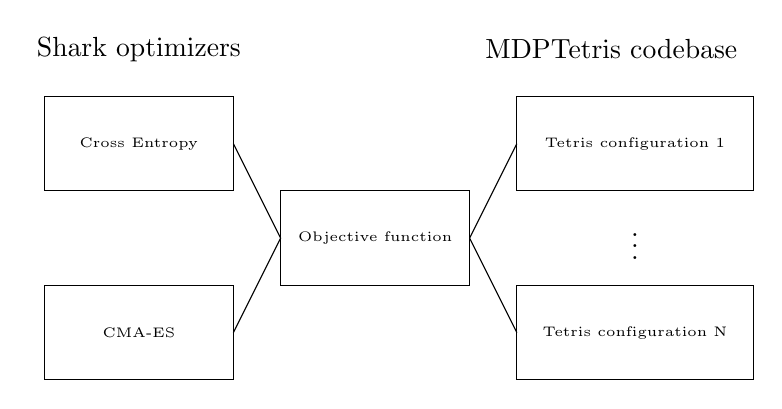
\begin{tikzpicture}[scale=0.6]
\draw  (0,0) rectangle (4,2);
\node at (2,1) {\tiny Objective function};
\draw  (-5,4) rectangle (-1,2);
\node at (-3,3) {\tiny Cross Entropy};
\draw  (-5,0) rectangle (-1,-2);
\node at (-3,-1) {\tiny CMA-ES};
\draw  (5,4) rectangle (10,2);
\draw  (5,0) rectangle (10,-2);
\node at (7.5,1) {$\vdots$};
\node at (7.5,3) {\tiny Tetris configuration 1};
\node at (7.5,-1) {\tiny Tetris configuration N};
\draw (-1,3) -- (0,1) -- (-1,-1);
\draw (5,3) -- (4,1) -- (5,-1);
\node at (-3,5) {Shark optimizers};
\node at (7,5) {MDPTetris codebase};
\end{tikzpicture}
\end{center}
\caption{Fusion of Shark and MDPTetris}
\end{figure}


The source code of the MDP-Tetris source code 
is accompanied with files that describe the
various existing features, that is files that defines 
the commonly used feature sets. As described, these files contains the identifiers of 
each feature to use, as well as two numbers respectively describing 
the agents reward function and how to evaluate a 'game over' state. 
The number for the reward function has remained unchanged at $0$ 
during all experiments. The "game-over" evaluation was for the
Bertsekas feature set initially set to $0$. Setting the 
"game-over" evaluation to $0$ means that the agent will not 
distinguish between regular moves and moves that results in losing
the game. If this setting remains at 0, the agent will always consult the
feature functions to rank it's moves, yet setting this value to $-1$
the agent will always, regardless of feature functions, rank moves that ends
the game the lowest.
When running the experiments with this setting as $0$, a large portion
of the agents never exceeded a zero mean score. This occurs presumingly 
due to all agents failing quickly giving the optimization algorithm no 
useful feedback. However, setting the value
to $-1$, meaning that a "game-over" move yields $-\infty$ reward, 
none of the experiments got stuck on only zero scores. An example
of the layout of the feature file can be seen in figure \ref{fig:featfile}.
\begin{figure}[h!]
\centering
\begin{lstlisting}
0    <- Describes the reward function
-1   <- Actions leading to game over is avoided at all cost
22   <- The policy contains 22 features
8 0  <- The feature with id 8 initially has weight 0
...  <- The remaining 21 features
\end{lstlisting}
\caption{Example of a file that describes a feature set. \label{fig:featfile}}
\end{figure}

\subsubsection{Game complexity \label{HardTetris}}
In order to reduce the runtime of experiments, to allow us more experiments in the evaluations, we can increase the "difficulty" of Tetris, by adjusting either the board size and/or adjusting the frequency of certain pieces. This has also been described before by Amine Boumaza, \citep{boumaza2009}.\\
To increase the difficulty of the game,
in our "Hard" Tetris, the s-block and z-block appear twice as often 
as the other pieces.

\begin{figure}[H]
\begin{center}
\includegraphics[scale=0.6]{img/Pieces}
\end{center}
\caption{Regular Tetris pieces \label{fig:TetrisPieces}}
\end{figure}

We want to test whether the game complexity has an impact on the performance of the algorithms,
therefore we want to test the two algorithms with Bertsekas/Tsitsiklis featureset, using Normal Tetris and Hard Tetris.\\

\textbf{Results}\\
In the following figure is depicted the mean results of 30 individual experiments using Cross Entropy and CMA, applied to both Hard Tetris and Normal Tetris. The general settings of the experiments can be seen in the appendix section, \ref{AppendixGameComplexity}.

\begin{table}[H]
\centering
\small
\begin{tabular}{l l r r r r r}
Tetris Type & Optimizer & mean & Q1 & Q2 & Q3\\
\hline
Hard & Cross Entropy & $1633.607$ & $1357.170$ & $1606.565$ & $1938.71$\\
Normal & Cross Entropy & $100059.463$ & $79357.440$ & $105999.500$ & $111047.500$\\
Hard & CMA & $449.352$ & $201.850$ & $300.300$ & $529.350$\\
Normal & CMA & $49760.161$ & $42528.740$ & $49915.700$ & $67764.729$\\
\end{tabular}
\caption{Experiment testing game Normal Tetris against Hard Tetris}
\end{table}

\begin{figure}[H]
\centering
\includegraphics[scale=1]{data/complexity/mean/PlotFile.pdf}
\caption{Experiment testing Normal Tetris against Hard Tetris}
\end{figure}

\textbf{Analysis and discussion}\\
The results indicate that using Hard Tetris does not impact the general development of the algorithms, meaning we are able to use the harder Tetris for further experiments. From the graph it appears that the harder Tetris simply shifts the score compared to normal Tetris.
\\


\subsubsection{Comparison of featuresets  \label{compoffeatureset}}
As described in section \ref{prevWork}, there are different kind of featuresets which
impacts the performance of the agents. In our upcoming experiments, we are going to
use both the Dellacherie and Bertsekas/Tsitsiklis featureset. For our initial comparison experiments
we are going to use the Bertsekas/Tsitsiklis featureset, since other researchers report
a lower score with the Bertsekas/Tsitsiklis featureset compared with the Dellacherie featureset
\citep{thiery:09}. Compared to the \citep{thiery:09} experiments, we don't want to maximize the
final score, but rather maximize the score with the lowest possible number of 
games evaluated.\\
It's important to note that we are not going to conduct comparison experiments with different
featuresets in the same experiment, since the algorithms needs to be on equal terms.\\
\\
We want to test whether the featureset has an impact on the performance of the algorithms,
therefore we want to test the two algorithms with both the Dellacherie and Bertsekas/Tsitsiklis featureset.\\
From the game complexity section \ref{HardTetris}, we have verified that using Hard Tetris
\citep{boumaza2009} does not have an impact on the development of the two algorithms.
Therefore, to prevent long runtimes, the games were simulated
using Hard Tetris.\\

\textbf{Results}

In the following figures the mean results of 30 runs of both CMA and Cross 
Entropy is presented. The settings for Cross Entropy remains at constant noise
with a noise term of $z_t = 4$ and an initial sigma of $\sigma_0 = 100.$, 
and the CMA with $\sigma_0 = 1$.\\
\\
Figure \ref{fig:featuresetCompareBertsekas} shows the experiment with the 
Bertsekas featureset. This shows that when running the algorithms with a
harder game, the algorithms behave mostly the same as with regular 
Tetris. Namely that CMA converges faster than Cross Entropy, 
but is eventually outperformed.

\begin{figure}[H]
\includegraphics[scale=1]{plots/plotBertsekasCmaVsCEHardTetris}
\caption{Comparison between CMA-ES and Cross Entropy 
using hard Tetris and the Bertsekas featureset 
\label{fig:featuresetCompareBertsekas}}
\end{figure}

When using the Dellacherie featureset a similar behaviour is observed.
However, the convergence seems to occur earlier and with a higher score
(figure \ref{fig:featuresetCompareDellacherie}).

\begin{figure}[H]
\includegraphics[scale=1]{plots/plotDellCmaVsCEHardTetris}
\caption{Comparison between CMA-ES and Cross Entropy 
using hard Tetris and the Dellacherie featureset
\label{fig:featuresetCompareDellacherie}}
\end{figure}

\textbf{Analysis and discussion}

The experiment with different featuresets indicates that the behaviour 
is not heavily dependant on the featureset.
It appears that changing the featureset simple shifts the score, but does not affect the development of the graphs.\\
Therefore, we conclude that changing the featureset does not invalidate
the comparison of the two optimization algorithms.



\subsection{Setup}

When executing the experiments, various parameters each have 
an impact on the final result of the learning curve. Thus, the parameters
are adjusted, first to match the experiments run by other researchers, 
and later to conduct as fair as possible comparisons between 
Cross-Entropy and CMA-ES.\\
\\
% agents
The amount of vectors sampled in each generation $\populationSize$
has a high impact on the algorithm performance. By setting $\populationSize$
high, more policies are evaluated per iteration, and leads to a more thorough 
exploration of the search space. Thus the higher $\populationSize$ increases the
chances of finding a better mean for the next iteration.
However, higher $\populationSize$ also results in the
need for more evaluations per iteration. The goal for 
tuning this parameter is then
to set $\populationSize$ high enough to ensure 
exploration of good solutions, and yet 
low enough to avoid unnecessary evaluations.\\
In the implementation of CMA-ES from \shark , 
the algorithm  itself determines
the value of $\populationSize$ according to the 
size of the search space. 
Cross-Entropy however, does not seem to have a 
general rule for this parameter,
so this value is manually adjusted to fit the 
problem as well as possible.\\
\\
% offspring
As both of the optimizing algorithm uses a subset of the sampled vectors
from a generation to update the distribution parameters, the number of 
offspring $\offspringNumber$ influences how the next generation is sampled.
By setting the value too high, the algorithm risks ceasing to progress any 
further since the updated mean would be too close to the previous one to 
significantly make a difference. By setting the value too low,
the risk of reaching a local optimum increases since the high-scoring agents
might have reached their high performance by chance.\\
The CMA-ES itself manages setting $\offspringNumber$ and Cross-Entropy
is set according to the problem. Most authors that uses Cross-Entropy for Tetris
sets the offspring size to $10\%$ of population size, that is 
$\offspringNumber = \lfloor 0.1 \cdot \populationSize \rfloor $.\\
\\
% Number of games per iteration
The number of games, $\numberOfEvaluations$, 
is the number of games  which each agent 
plays in each iteration. An agent's score is defined as the 
mean of the score of these 
$\numberOfEvaluations$ games.
We want this value low as possible, because as with the number of
agents, $\populationSize$, The number of games, $\numberOfEvaluations$, 
is another major factor in the run-time of the algorithm.
As Tetris is stochastic by nature, the score deviates a lot, 
even when the
same agent with the same policy plays multiple games. 
Hence, when assessing the true
performance of a policy it's rarely enough to play just few games. Thus, setting 
$\numberOfEvaluations$ high increases the likelihood of correctly choosing the best 
agents, yet, it also causes longer run times of the experiments.\\
\\
% Noise factor
Specific to the Cross-Entropy method, 
most authors report that the performance of the 
algorithm increases dramatically when the sampling 
distribution is associated with
a noise term. The different types of 
noise are described in section \ref{CrossEntropy}.
The noise term is adjusted in order to 
prevent the algorithm from reaching a local optimum.
The current research shows that noise terms of $\noise_\generation = 4$ and 
$\noise_\generation = max \left( 5 - \generation / 10 \right)$ 
\citep{thiery:09} produces the best results.
The constant noise (such as $\noise_\generation = 4$) ensures that the algorithm
never settles in a too small area from which it samples, and forces it to explore
solutions that are further away from the mean. The further the 
algorithm progresses, 
the less noise is assumed needed, as the mean should approach a global optimum. to
address this, the linear decreasing noise 
is applied as it will lower the noise term
as the algorithm progresses.\\
\\
For the various experiments, these 
parameters will be tuned for the specific purpose 
at hand. In the verification of the Cross-Entropy, the parameters are set 
to match those reported in similar papers (\cite{thiery:09}, \cite{szita:06}).
In the comparison of the two algorithms, the parameters will be set such that 
the Cross-Entropy operates under as 
similar conditions as CMA-ES, to ensure an unbiased 
comparison.







\subsection{Verification of our implemented Cross Entropy \label{varifyofce}}

Because the \shark library already contains an implementation of 
CMA-ES, but not an implementation of Cross Entropy, we extended the library 
with our own implementation of the algorithm.\\
In order to verify the correctness of the implementation, 
we used the same experiments as used by 
Christophe Thiery and Bruno Scherrer \citep{thiery:09}. 
These experiments were used by Thiery and Scherrer to 
verify their own Cross Entropy implementation with various types of noise correction. 
Therefore, we will perform the same experiments to verify our 
own contribution to the \shark library, by trying to achieve the same results.\\
\\
The setup is mirrored from the paper \citep{thiery:09}, 
with 100 agents ($\populationSize = 100$) per iteration,
and using the $\offspringNumber = 10$ best vectors
for the update step. After each iteration, 
an agent with the updated mean 
plays 30 games and the mean of these scores are recorded for the
learning curve.\\
During evaluation each agent plays one game, that is $\numberOfEvaluations = 1$.
A minor derivation from the figures present in \citep{thiery:09}, is 
the unit along the x-axis in the learning curve plots indicates 
the iteration number. As the experiments in this two algorithms
width variable population sizes are compared, the x-axis in all plots
indicated the number of tetris games played during the learning. In one 
generation $\populationSize$ agents each play $\numberOfEvaluations$ games and hence
adavance the x-axis by $\populationSize \numberOfEvaluations$.\\

\begin{figure}[H]
\begin{center}
\includegraphics[scale=0.8]{plots/meansPlot}
\end{center}
\caption{Cross-Entropy mean performance \label{fig:cemean}}
\end{figure}

\clearpage
\begin{figure}[H]
\begin{center}
\includegraphics[scale=0.48]{plots/noNoisePlot}
\end{center}
\caption{No noise \label{fig:ceNoNoise}}
\end{figure}
\begin{figure}[H]
\begin{center}
\includegraphics[scale=0.48]{plots/constantNoisePlot}
\end{center}
\caption{Constant noise \label{fig:ceCnstantNoise}}
\end{figure}
\begin{figure}[H]
\begin{center}
\includegraphics[scale=0.48]{plots/linearNoisePlot}
\end{center}
\caption{Linear decreasing noise \label{fig:ceLinNoise}}
\end{figure}

Figure \ref{fig:ceNoNoise}, \ref{fig:ceCnstantNoise} and
\ref{fig:ceLinNoise} shows 10 runs of each noise type. Figure
\ref{fig:cemean} shows the mean graph for each of the noise types.
The goal of these experiments were to replicate the experiments 
reported in \citep{thiery:09}. As the results seen from our experiments
to a high degree resemble those reported by Thiery et. al, we conclude
that our Cross Entropy implementation works similar to theirs.\\
\\
When evaluating the score of the agent we also want to compute the confidence
interval in verifying the implementation of Cross Entropy. The mean agent plays 30 games
which leads to a confidence interval of $\pm36\%$ around the estimated mean,
which is similar to the confidence intervals in \citep{scherrer2009}.\\
By looking at the individual graphs for the different noise types 
(Figure \ref{fig:ceNoNoise}, \ref{fig:ceCnstantNoise} and
\ref{fig:ceLinNoise}), we get the following average scores.\\
\\
\textbf{Without noise (figure \ref{fig:ceNoNoise})}: The learning curve
stabilizes after 1,500 agents evaluated. And as it can be observed the
score variates much for the different executions between a score of 300 and 6,000
rows. This results in an average score of 1,400$\pm36\%$ rows.\\
\textbf{Constant noise (figure \ref{fig:ceCnstantNoise})}: 
The 10 executions reaches equivalent performances at some point, 
with a score between
54,000 and 154,000. This results in an average score of 105,000$\pm36\%$ rows.\\
\textbf{Linear decreasing noise (figure \ref{fig:ceLinNoise})}:
Most of the executions of this noise type settles around 200,000.
However, a single execution settled at a score of only around 5,000.
The mean performance of this noise type yielded a score of
120,000$\pm36\%$ \\

Based on the mean graphs and confidence interval compared to other papers, we can
hereby verify that our implementation of Cross Entropy works as intended. Even though the
experiments with linear decreasing noise in this case seems to outperform
the constant noise, other runs with linear decreasing noise ended in a mean 
performance of only 90,000$\pm36\%$. Yet, the constant noise is both from our
own experiments, and described in other research, noted to be the most reliable
noise type for reaching high scoring controllers \citep{scherrer2009}. 
Due to this, the constant noise is used in the 
benchmarking against CMA.\\





\subsection{Optimal settings 
for Cross Entropy \label{optimalsettingsce}}

In this section we will determine the optimal settings for Cross Entropy through testing
of various adjustable parameters.\\
Compared CMA, Cross Entropy has fewer customizable parameters, more specifically 
population-parent size and games played per agent.

\subsubsection{Population and selection size}

Other researchers run the Cross Entropy algorithm with population size of
$\populationSize = 100$ and an offspring corresponding to 10\% of 
the population size, resulting in $\offspringNumber = 10$. As it's not 
discussed why this exact setting is applied, various settings of the 
Cross-Entropy was executed to asses the performance of other configurations
in our experiments.
The experiments includes different population sizes 
$\populationSize \in \{10, 22, 50, 100, 200\}$ and offspring 
sizes of either $10\%$ and $50\%$ (since the CMA algorithm by default
uses $50 \%$ selected vectors). 
A summary of the experiments can be seen in figure \ref{CEConfigTest}
on page \pageref{CEConfigTest}.

\begin{figure}[H]
\centering
\begin{tabular}{r r | r r r r}
$\populationSize$ & $\offspringNumber$ & mean & Q1 & Q2 & Q3\\
\hline
10 & $10\%$  & 704.6      & 7.2       & 48.3         & 430.3\\
10 & $50\%$  & 9,272.5    & 149.6     & 7626.5       & 16,919.9\\
22 & $10\%$  & 35,841.6   & 20,391.9  & 42,045.5     & 48,464.6\\
22 & $50\%$  & 52,887.4   & 23,531.9  & 42,161.0     & 83,144.1\\
50 & $10\%$  & 95,623.1   & 82,738.9  & 93,388.9     & 111,351.5\\
50 & $50\%$  & 69,130.7   & 52,511.0  & 64,351.6     & 91,488.6\\
\hdashline
100 & $10\%$ & 115,868.7  & 84,368.5  & 122,238.5    & 146,457.0\\
\hdashline
100 & $50\%$ & 22,910.4   & 4,037.7   & 14,353.7     & 47,215.9\\
200 & $10\%$ & 85,181.7   & 45,201.5  & 96,803.1     & 117,578.0\\
200 & $50\%$ & 946.4      & 585.0     & 802.5        & 1,267.7
\end{tabular}
\caption{Cross Entropy configuration test, 
see Appendix \ref{appendixCrossEntropyConfig} for the full plots 
of the experiments.  \label{CEConfigTest}}
\end{figure}

The experiments with different population and parent sizes
does not seem to support a choice for any other configuration 
than the mostly commonly used 
$\populationSize = 100$ and $\offspringNumber = 10$. \\
However, with a configuration of $\populationSize = 50$ and $\offspringNumber = 5$ convergence
is achieved faster (see figure \ref{fig:bestConfCE}). This means that the score limit is reached faster, which
results in longer computation time, than the $\populationSize = 100$ and $\offspringNumber = 10$
configuration. In other words, the $\populationSize = 100$ and $\offspringNumber = 10$ configuration 
is therefore preferred since it takes shorter computation time and the end-result is similar compared
to the $\populationSize = 50$ and $\offspringNumber = 5$ configuration, even though the latter 
configuration from our expriments converged faster. The experiments also apppears
to suffer from a high noise, yet both the mean and the quantiles favor the 
extensively tested Cross Entropy configuration of $\populationSize = 100$ and $\offspringNumber = 10$.


\begin{figure}[H]
\begin{tabular}{@{}l@{}l@{}}
\includegraphics[scale=1]{plots/ce_ConstantNoise_l50_o5_all} &
\includegraphics[scale=1]{plots/ce_ConstantNoise_l100_o10_all}
\end{tabular}
\caption{The two best configurations of Cross Entropy 
\label{fig:bestConfCE}}
\end{figure}

\subsubsection{Games per agent \label{GamesPerAgentCESection}}

Another parameter we can adjust is the number of 
games played each agent plays per generation. By playing
multiple games with each agent and using their 
mean score to compute the next generation mean. This
secures a higher chance of a better offspring generation,
but at the cost of more games
evaluated.\\
Table \ref{GamesPerAgentCE} shows the different values of
games per agent we are going to be
testing.

\begin{table}[H]
\centering
\begin{tabular}{c c c}
Population Size & Parent size & Games per Agent\\
\hline
$12$ & $10\%$ & 1/3/5/7/10\\
$12$ & $25\%$ & 1/3/5/7/10\\
$12$ & $50\%$ & 1/3/5/7/10\\
$22$ & $10\%$ & 1/3/5/7/10\\
$22$ & $25\%$ & 1/3/5/7/10\\
$22$ & $50\%$ & 1/3/5/7/10\\
$50$ & $10\%$ & 1/3/5/7/10\\
$50$ & $25\%$ & 1/3/5/7/10\\
$50$ & $50\%$ & 1/3/5/7/10\\
$100$ & $10\%$  & 1/3/5/7/10\\
$100$ & $25\%$  & 1/3/5/7/10\\
$100$ & $50\%$ & 1/3/5/7/10\\
$200$ & $10\%$ & 1/3/5/7/10\\
$200$ & $25\%$ & 1/3/5/7/10\\
$200$ & $50\%$ & 1/3/5/7/10
\end{tabular}
\caption{Games per agent CE experiment setup\label{GamesPerAgentCE}}
\end{table}

The experiments includes different games per agent of $\{1,3,5,7,10\}$. By increasing the number of games 
played per agent, we are increasing the evaluation cost by a multiplication factor in exchange for a more 
accurate evaluation of each agent. This is to avoid misconceiving poor performing agents
for good ones, as multiple evaluations will decrease the chance the agent having 
'lucky games'. However, we wish to find 
the best performing configuration with the lowest cost and maximum benefit, and evaluating multiple 
times will increase the function cost.\\
\\
\textbf{Results}\\
The total number of configuration experiments is 75, with 30 individual experiments each,
resulting in a total of 2.250 individual experiment runs. These results are all included in 
appendix \ref{appendixCEPopulationParent}.\\
Below in table \ref{CEBestConfigTable} and figure \ref{CEBestConfigPlot}, the five best
best resulting configurations are depicted. We chose these by first selecting the best 
configuration of each Population-Parent size. This results in three
configurations for each Population-Parent size, which we then compare to determine the best
configuration for each Population-Parent size. Which is depicted in table \ref{CEBestConfigTable} and figure \ref{CEBestConfigPlot}.
\begin{table}[H]
\centering
\small
\begin{tabular}{c c c r r r r}
Population & Parent & Games per Agent & mean & Q1 & Q2 & Q3\\
\hline
$12$ & $6$ & 10 & $2109.837$ & $1802.968$ & $2021.165$ & $2276.652$\\
$22$ & $5$ & 5 & $2371.793$ & $2013.168$ & $2412.815$ & $2708.931$\\
$50$ & $12$ & 5 & $2749.991$ & $2605.171$ & $2702.400$ & $2835.960$\\
$100$ & $25$ & 3 & $2776.560$ & $2397.691$ & $2742.950$ & $3027.541$\\
$200$ & $50$ & 1 & $2950.767$ & $2564.118$ & $2841.065$ & $3377.189$\\
\end{tabular}
\caption{Best configurations of all population sizes - Cross Entropy \label{CEBestConfigTable}}
\end{table}

\begin{figure}[H]
\centering
\includegraphics[scale=1]{data/ce_population_offspring/bestofall_population/PlotFile.pdf}
\caption{Best configurations of all population sizes - Cross Entropy \label{CEBestConfigPlot}}
\end{figure}

From table \ref{CEBestConfigTable} and figure \ref{CEBestConfigPlot}, we can see that population size 50 with parent size 12 and 5 games per agent, population size 100 with parent size 25 and 3 games per agent, and, population size 200 with parent size 50 and 1 game per agent, performs almost identically.\\\\

\textbf{Discussion and analysis}
\comment{pick best of three configurations and determine why}


\subsection{Optimal settings 
for CMA \label{optimalsettingscma}}

When finding the optimal settings for CMA we have a larger set of parameters we can adjust compared
to Cross Entropy. Again, as the same with Cross Entropy, we can adjust the population/parent size and
games per agent. Furthermore we can adjust the initial step-size, lower bound and recombination type.\\
The following sections will go into detail how these parameters affect the performance of CMA
algorithm. In the last section we will perform experiments to determine the optimal settings.

%In previous sections we focused on tuning Cross Entropy for the Tetris 
%problem. Whereas we deliberately chose not to tune CMA due to its implementation 
%into the Shark library \citep{shark08}. However, experiments with the "out of 
%the box" CMA from Shark, with default settings vs the tuned Cross Entropy
%resulted in CMA reaching convergence very fast but not achieving the same point
%limit as Cross Entropy.\\

\subsubsection{Recombination type}
Furthermore, CMA also has a unique formula for calculating the updated mean,
called the 'Recombination type' \ref{CMAtheory}. Where the recombination type
determines how much influence each of the offspring vectors has on the next
generation. Built into the CMA algorithm is three methods of recombination. 
\begin{itemize}
\item EQUAL, Each of the offspring vectors has equal influence in the generated mean. Each has $w_i = 1$.
\item LINEAR, The best of the offspring vectors has more influence. 
\item SUPERLINEAR, The vectors are weighted with a logarithmic equation. $w_i = \frac{w_i'}{\sum_{j=1}^{\mu} w_j'^+}$
\end{itemize}
As default, CMA uses Super Linear recombination. However, Tetris is a problem
with multiple local optimums in its solution space. This means, though a vector may be the best in its generation, it could be a nearby local optimum. Therefore, Super Linear recombination may not be the optimal recombination type for the Tetris problem.\\

\comment{- Weights for recombination could have a symbol? (change policy weight
symbol?)}\\
\comment{- Find Linear combination type formula of change format of itemize list}

\subsubsection{Population and selection size}
By adjusting the population size to that similar of Cross Entropy, we are able
to get a fair comparison between the two algorithms, given each generation will
contain the same number of agents. By setting the population and parent size
to the same values, we in effect test if the covariance matrix and the step-size
control has a impact on the algorithm performance compared to Cross Entropy
which does not have the features.\\
Table \ref{CMAPopulationSelectionConfigTest} displays the values that we are going
to test for the population and selection size.

\begin{table}[h]
\centering
\begin{tabular}{c c}
Population size, $\populationSize$ & Parent size, $\offspringNumber$\\
\hline
$12$ & $1$\\
$12$ & $3$\\
$12$ & $6$\\
$22$ & $2$\\
$22$ & $5$\\
$22$ & $11$\\
$50$ & $5$\\
$50$ & $12$\\
$50$ & $25$\\
$100$ & $10$\\
$100$ & $25$\\
$100$ & $50$
\end{tabular}
\caption{CMA configuration for population and parent size \label{CMAPopulationSelectionConfigTest}}
\end{table}

The experiments includes different population $N \in \{12,22,50,100\}$ and offspring sizes of either
10\%, 25\% and 50\%. We use 10\% because of the Cross Entropy recommended selection size, while
we use 25\% because of CMA's standard selection size for the EQUAL recombination type. 
Furthermore we use 50\% because of CMA's standard selection size for the LINEAR and SUPERLINEAR 
recombination type.

\subsubsection{Games per agent \label{CMAGamesPerAgentSection}}
As with Cross Entropy we can also adjust the number of games each agent plays per generation.
However, because of the recombination type for CMA, one game pr. agent may  be insufficient to assess the
performance of an agent. The Linear and Super Liner recombination types will value the better agents higher.
Therefore, it may occur that some better-on-average agent encounter an unlucky game, achieving a lower score than
it's actual potential allows. \\
Thus, evaluating each agent multiple times and using the average score for recombination may allow for a more accurate assessment.\\
Table \ref{CMAGamesPerAgent} displays the values that we are going
to test for games per agent.

\begin{table}[h]
\centering
\begin{tabular}{c}
Games per agent\\
\hline
$1$\\
$3$\\
$5$\\
$7$\\
$10$
\end{tabular}
\caption{CMA configuration for games per agent \label{CMAGamesPerAgent}}
\end{table}

The experiments includes different games per agent of $\{1,3,5,7,10\}$. We have chosen the same 
values as with Cross Entropy to get comparable results (see section \ref{GamesPerAgentCESection}).

\subsubsection{Initial step-size}
Initially, the covariance matrix of CMA in generation $\generation = 0$
is the identity matrix. The initial step-size, $\sigma_0$, will hence in 
the first iteration scale the area in which the CMA algorithm searches.
As from section \ref{normalSamples}, it's known that the scale of the 
solutions has no impact on the scores. Hence, it's assumed that the initial 
step-size should not have any major impact on the results.

\begin{figure}[H]
\centering
\begin{tabular}{r | r r r r r}
$\sigma_0$ & mean & Q1 & Q2 & Q3\\
\hline
0.1 & 50769.3 & 21301.1 & 54588.7 & 73972.4\\
0.2 & 42290.6 & 32180.2 & 42290.6 & 49337.4\\
0.5 & 53893.7 & 14211.1 & 66773.0 & 85816.7\\
0.8 & 37557.7 & 1422.8  & 15450.8 & 93719.4\\
1.0 & 49537.9 & 31369.8 & 49537.4 & 58454.6
\end{tabular}
\caption{Results of CMA-ES with adjusted initial step-size \label{CMAInitialSigmaConfigTest}}
\end{figure}

\comment{Add the data-graphs to appendix}

For the initial experiments using CMA-ES, 
the only adjusted parameter is the initial 
step-size $\sigma_0$. The configurations of step-sizes were 
$\sigma_0 \in \{0.1, 0.2, 0.5, 0.8, 1.0\}$. As the table shows,
the final mean score does not seem to change with the initial step-size.
Furthermore, the adjustment of the step-sizes does not appear to 
have a drastic impact on the mean scores. However, based on both mean score and
quantiles, the best configuration seems to be $\sigma_0 = 0.5$. This is 
is also referred to as a typical initial setting in \citep{boumaza2009}.
Therefore, the conclusion remains that the initial step-size is not critical 
for the experiment.\\

\comment{- Make sure to fully conclude that the initial step-size doesn't matter and therefore we don't
use this paramater in the upcoming experiments}

\subsubsection{Lower bound}

As with the Cross Entropy method, to avoid too early convergence, a 
certain lower threshold for the variance should be applied when 
sampling vectors for solutions. In the Cross Entropy method, a constant 
noise term $z_t = 4$ was added to the variance for each component
of the sampled vectors. When the $i$'th component in cross entropy is
sampled as follows
\begin{align*}
\individual_i &\sim \mathcal{N}\left(m, \sigma^{2}\right)\\
              &\sim \sigma \mathcal{N}\left(m, 1\right)
\end{align*}
Then $\sigma^{2} \geq 4$. To gain the same effect for the CMA, a lower bound 
is applied to the step-size. Such a bound is implemented in the Shark library
as the following, where the value of the lower bound is $l$.
\begin{align*}
\sigma  \lambda_n \geq l
\end{align*}
Where $\lambda_n$ is the lowest eigenvalue in the covariance matrix. 
When the vectors are sampled, the samples are scaled by the matrix $D$
containing the eignvalues of the covariance matrix. 
Hence, if $\sigma \lambda_n \geq l$, then the smallest scaling
that takes place is at least $l$. As the vectors are sampled
as
\reminder{Check if this is correct, 
and maybe place this in theoretical section.
Also make sure that variable names makes sense.}
\begin{align*}
\individual &\sim \mathcal{N}\left( m, \sigma^{2}C \right)
\end{align*}
To roughly resemble the constant noise configuration of Cross Entropy,
the dimension with the lowest variance must not drop below 4. 
This is achieved by setting a lower bound $l=2$. By setting this, 
the variance of the normal distribution in each dimension 
before rotation is ensured to be at least $\sigma^{2} = 4$
since $\sigma \mathcal{N}\left( 0, 1 \right) \sim 
\mathcal{N}\left( 0, \sigma^{2} \right)$.


\maybe{From this, it's assumed that the initial step-size, at least in this range,
does not have a significant impact, and the best of these runs, $\sigma_0$ is chosen
for first comparison.}
\comment{- Write stuff about our practical experiences with lower bound and add the graphs to appendix}\\
\comment{- Make sure to fully conclude that the lower bound doesn't matter and therefore we don't
use this paramater in the upcoming experiments}

\subsubsection{Experiment for finding the optimal settings}
In this in section we are going to conduct a wide variety of experiments to determine
the best settings for CMA. More specifically we are going to find the best combination for
population size, parent size and games per agent.\\
Table \ref{SuperCMAExperiment} shows the different experiments we are
going to carry out.

\begin{table}[H]
\centering
\begin{tabular}{c c l c}
Population Size & Parent size & Recombination Type & Games per Agent\\
\hline
$12$ & $1$ & EQUAL/LINEAR/SUPERLINEAR & 1/3/5/7/10\\
$12$ & $3$ & EQUAL & 1/3/5/7/10\\
$12$ & $6$ & LINEAR/SUPERLINEAR & 1/3/5/7/10\\
$22$ & $2$ & EQUAL/LINEAR/SUPERLINEAR & 1/3/5/7/10\\
$22$ & $5$ & EQUAL & 1/3/5/7/10\\
$22$ & $11$ & LINEAR/SUPERLINEAR & 1/3/5/7/10\\
$50$ & $5$ & EQUAL/LINEAR/SUPERLINEAR & 1/3/5/7/10\\
$50$ & $12$ & EQUAL & 1/3/5/7/10\\
$50$ & $25$ & LINEAR/SUPERLINEAR & 1/3/5/7/10\\
$100$ & $10$ & EQUAL/LINEAR/SUPERLINEAR & 1/3/5/7/10\\
$100$ & $25$ & EQUAL & 1/3/5/7/10\\
$100$ & $50$ & LINEAR/SUPERLINEAR & 1/3/5/7/10
\end{tabular}
\caption{Full experiments overview \label{SuperCMAExperiment}}
\end{table}

The choice behind using the above population sizes is to use the same population sizes as
when we tuned Cross Entropy (see section \ref{optimalsettingsce}). However, we use a population
size of 12 instead of 10, because a population size of 12 is the stock setting for Shark CMA \citep{shark08}.\\
In regard to the parent size, they have been determined depending on the recombination type.
We use all three different recombination types for the 10\% parent sizes to make these experiments
correspond to the Cross Entropy settings (see section \ref{optimalsettingsce}). However, Shark CMA
has predetermined parent sizes for each recombination types, 25\% for EQUAL and 50\% for both
LINEAR and SUPERLINEAR \citep{shark08}. For this reason we also conduct experiments for each population
size to represent these Shark CMA preferred settings.
Furthermore we also test different number of games per agent as for the reason presented in section
\ref{CMAGamesPerAgentSection}.\\

\textbf{Results}\\
\comment{show results, specify best resuslts/candidates.}\\

\textbf{Analysis and discussion}\\
\comment{Discuss best results/candidates and conclude the optimal settings.}\\











\subsection{Comparison between Cross Entropy and CMA}

\comment{- Some kind of introduction which states that this entire section is written 
"chronological"}\\
\comment{- In each experiment, make sure to state which paramters we use/adjust and what we don't
adjust}

\subsubsection{Global comparison settings}
In all papers used for reference we haven't seen any experiments with different population
and parent sizes presented side-by-side. All the experiments we've seen
that has applied Cross Entropy to Tetris fix the population size to 100. 
However, in our upcoming experiments
CMA and CE are configured with different population and parnet numbers, which means
that we cannot compare the learning curves based on iterations/generations. Instead as described
in section \ref{varifyofce}, using the  
\textit{number of games played} as comparison reference, equal terms are secured for both algorithms 
in regards to learning speed. \\
Hence x-axis shows the total number 
of Tetris games evaluated, 
$\sum_{i = 1}^{\generation} \populationSize \numberOfEvaluations$. 
Meanwhile the y-axis still represents the mean score 
of the centroid agent at iteration $\generation$.

\subsubsection{Initial comparison - Default settings \label{sec:initialCompare}}
The initial comparison is meant to show how the CMA-ES performs against the Cross-entropy method
under default settings. The default setting for CMA-ES are those set by default
by Shark. The settings for the Cross-entropy method are those that are said to perform best
and most
consistently by other researchers.
Hence, the goal of this comparison is to get an initial 
idea of how the Shark implementation of
CMA-ES compares to the Cross-entropy method with settings
used by other researchers \citep{thiery:09}. Table \ref{tab:initialComparisonSettings}
summarises the settings of each algorithm used in the initial experiment.
\begin{table}[H]
\centering
\begin{tabular}{l r}
Optimizer & CMA-ES\\
Evaluations/agent & 8000\\
Learning Games & 30\\
Population size& 13\\
Parent size & 6\\
Games per Agent & 1\\
Tetris Type & Normal\\
\hline
Recombination Type & SUPERLINEAR\\
Initial Sigma & 0.5\\
Lower bound & NONE\\
\end{tabular}
\quad
\begin{tabular}{l r}
Optimizer & Cross Entropy\\
Evaluations/agent & 8000\\
Learning Games & 30\\
Population size & 100\\
Parent size & 10\\
Games per Agent & 1\\
Tetris Type & Normal\\
\hline
Sigma & 100\\
Noise Type & Constant\\
Noise & 4
\end{tabular}
\caption{Optimized Cross-entropy method and CMA-ES for comparison experiments \label{tab:initialComparisonSettings}}
\end{table}


\textbf{Results}

Figure \ref{fig:CMA_VS_CE_00} shows the mean learning curves of the two algorithms,
and table \ref{table:initialResultTable} shows the results from the final iteration of each algorithm.
As figure \ref{fig:CMA_VS_CE_00} reveals that CMA-ES converges faster,
but reaches a local optimum at around 2,000 games played. Meanwhile the Cross-entropy method has a 
slower convergence but reaches a better mean score compared to CMA-ES at around 5,500
agents evaluated. In detail, CMA-ES on average reaches a score of 50,000 rows, and
the Cross-entropy method reaches a score of 100,000.\\

\begin{figure}[H]
\begin{center}
\includegraphics[scale=0.8]{plots/cmaCePlot}
\end{center}
\caption{Initial comparison between CMA-ES and Cross-entropy method \label{fig:CMA_VS_CE_00}}
\end{figure}

\begin{table}[H]
\centering
\small
\begin{tabular}{l r r r r}
Optimizer & Mean & Q1 & Q2 & Q3\\
\hline
CMA-ES  & $57783.0$ & $10269.9$ & $59774.5$ & $100384.1$\\
The Cross-entropy method & $116289.4$ & $85230.9$ & $125329.5$ & $138715.5$\\
\end{tabular}
\caption{Results from last iteration of the curves in figure \ref{fig:CMA_VS_CE_00}
\label{table:initialResultTable}}
\end{table}

\textbf{Analysis and discussion}

These results clearly defy our initial hypothesis as we predicted
for CMA-ES to outperform Cross-entropy method, due to its more sophisticated nature. 
One reason for this outcome could possibly be that
CMA-ES has a very little population size compared to Cross-entropy method,
which could be a decisive lack as the objective function is noisy with 
a high variance.\\

\begin{changebar}
To perform a comparison between the two algorithms on the same terms,
we saw from earlier experiments that both algorithms benefits from 
adjusted settings. Thus, another experiment is required, where both algorithms
are adjust to have the best possible settings to ensure that both algorithms
perform as well as possible. Among the adjusted parameters are the following.\\
\\
\textit{Enlargment of population size}\\
Our first experiment clearly shows that the CMA-ES
is outperformed by the Cross-entropy method.
The CMA-ES does by default only have a relatively small
population size (around 13) compared to the Cross-entropy methods
default (100). From the earlier experiments, we saw that 
the Cross-entropy method does benefit from a higher populations size,
and to CMA-ES, the higher population size appears critical
to it's performance. Thus, the population size is increased for 
both algorithm in our final experiment.\\
\\
\textit{Evaluate each agent multiple times}\\
From our experiments, the Cross-entropy method does not
seem to require evaluation each search point more than once
and thus, the number of evaluations remains at 1 per
search point. For the CMA-ES however, with a 
ranking mechanism that strongly emphasizes 
the best search points in a population, a firm
ranking is important. Our experiments suggested that
evaluation each search point 5 times appears to be optimal 
for the CMA-ES.\\
\\
\textit{Change the recombination type}\\
As described in section \ref{CMAtheory}, 
the CMA-ES is not bound to update its 
new mean to just the centroid of the selected 
vectors. Instead, it can weight better solutions
more heavily when moving its mean. When doing so,
it risks biasing search points that appear to be better 
but in reality, just by faulty ranking, should
not be considered a good agent. Our experiments 
did however suggest that with 5 evaluations per search agent,
the super linear recombination was the best option.\\
\\
None of the experiments seen so far has allowed a 
consistent mean score of more 
than 200,000. This brings the concern 
hat it might be the objective function
that poses a natural limit on the score into consideration.
In this case the objective function
models playing Tetris with the Bertsekas feature set. 
It is unknown to us
whether it's possible to construct an agent 
with a mean score of more than
200,000 lines on average. 
Thus we cannot know if convergence 
of the algorithms are caused by the feature set or limitations in the
algorithms.
\end{changebar}


\subsubsection{Tuned comparison - Optimized settings \label{tunedComparison}}
In this section we will conduct experiments comparing the optimized Cross Entropy Method 
against the
optimized CMA-ES obtained from the sections, \ref{GamesPerAgentCE} and \ref{OptimalSettingsCMA}.
The chosen optimal settings for each of the algorithms is specified in the following tables
\begin{table}[h]
\centering
\begin{tabular}{l r}
Optimizer & CMA\\
Number of Evaluations & 40000\\
Number of Learning Games & 30\\
Population size& 50\\
Parent size & 25\\
Games per Agent & 5\\
Tetris Type & Normal\\
\hline
Recombination Type & LINEAR\\
Initial Sigma & 0.5\\
Lower bound & 2.0\\
\end{tabular}
\quad
\begin{tabular}{l r}
Optimizer & Cross Entropy\\
Number of Evaluations & 40000\\
Number of Learning Games & 30\\
Population size & 200\\
Parent size & 50\\
Games per Agent & 1\\
Tetris Type & Normal\\
\hline
Sigma & 100\\
Noise Type & Constant\\
Noise & 4
\end{tabular}
\caption{Optimized Cross Entropy and CMA for comparison experiments}
\end{table}

\textbf{Results}\\

\begin{figure}[H]
\begin{tabular}{@{}c@{}c@{}}
Cross Entropy & CMA-ES\\
\includegraphics[scale=1]{plots/ce_tuned_all} &
\includegraphics[scale=1]{plots/cma_tuned_all}
\end{tabular}
\caption{30 experiment with optimal settings Cross Entropy Method and CMA-ES}
\end{figure}

\begin{figure}[H]
\centering
\includegraphics[scale=0.8]{plots/TunedPlot.pdf}
\caption{Mean plot of optimal settings Cross Entropy Method and CMA-ES}
\end{figure}


\textbf{Analysis and discussion}\\







\section{Conclusion}

To reach our goal of gathering empirical evidence to determine if either the Cross-entropy method
or the CMA-ES differ in performance when applied to Tetris, we implemented the Cross-entropy method in the Shark library and tested it against the pre-implemented version of the CMA-ES
algorithm. Our implementation of the Cross-entropy 
method has been accepted by the Shark development team, and is now part of the code base.
The widely used MDPTetris software was used to emulate the
Tetris games, and was used as the optimization problem for the optimization algorithms to solve.
The Cross-entropy method searches by using a Gaussian 
distribution, and therefore is stochastic in nature. Due to this, 
the verification of the algorithm was carried out as a comparison with other 
researchers' works of the same algorithm applied to the same problem, namely Tetris.\\
\\
After confirming that the Cross-entropy method does produce similar results as 
what we've seen in our references, we conducted an initial comparison between the
Cross-entropy method and the CMA-ES. The initial experiments used the default settings for CMA-ES
from Shark,
and the settings for the Cross-entropy method were the ones claimed to be optimal by other 
researchers. This initial experiment, revealed quite the opposite of our expectations 
according to our hypothesis, which was that the CMA-ES would outperform the Cross-entropy method
but at slower convergence. This experiment lead to the need of finding out whether the algorithms
could perform better with other settings. To find the better settings, a more difficult version
of Tetris was used to reduce the learning time of the algorithms. To thoroughly explore 
the impact of the different adjustable parameters more than 6,000 individual runs of the 
algorithms contributed to gain insight in how to best configure the two algorithms. These 
optimal settings were applied in a final comparison experiment.\\
\\
The results from the final experiment showed that a result that aligns better with our
hypothesis. The convergence of CMA-ES is heavily prolonged by the optimal settings
but does eventually reach scores that climbs slightly beyond those produced by the
Cross-entropy method. However, the final score of the two algorithms lies so close that
we cannot firmly differentiate between the two, and hence, cannot conclude that either of the
algorithms are better than the other. However, the results from our experiments 
suggests that the Cross-entropy method reaches its 
highest scores much faster than the CMA-ES under optimal settings, thus in conclusion
when learning Tetris using the MDPTetris platforms' approach, the Cross-entropy method 
stands out as the preferable choice.



\section{Future work}

\subsection{Noise handling}

Especially for the CMA-ES when using the superlinear recombination, the ranking of search
points is essential to the progression of the algorithm. As the score of the Tetris controllers
is under strong influence of noise, the CMA-ES can easily rank the 
candidate solutions wrongly. As controllers are conjectured and verified to
be exponentially distributed, the further the algorithm progress, the higher the likelihood
of faulty ranking. When the ranking becomes sufficiently unreliable, the CMA-ES will
no longer be able to tell which solutions are preferable and impair further progress
of the algorithm.\\
\\
One solution to this, which we have already used, is increasing the number of evaluations
performed on each search point. In our final experiment, the CMA-ES evaluated each agent
5 times to better distinguish between good and poor performing search points. This did turn out
to benefit the algorithm slightly, but at some cost. The high number of evaluations does not have a
significant effect at early stages. We saw that learning rate is quite high in during the first 
iterations but slows down as score, and therefore noise, increases. A simple solution
that we discussed  was to increase the number of evaluations based on iteration number.
A couple of ways to set 
\begin{align}
\numberOfEvaluations &=  \max\left( 1, k \lfloor \log_{2} \left( \generation \right)  \rfloor \right) &,\ k \in \mathbb{N}^+\\
\numberOfEvaluations &=  \max\left( 1, \left \lfloor{ \frac{\generation}{k} }\right \rfloor \right) &,\ k \in \mathbb{N}^+
\end{align}
This way, the number of evaluations increase with the iteration number, and should approximately
increase with the noise. This could help overcome the faulty ranking as noise gets higher.\\
\\
A more versatile solution to ensure good ranking is an approach described by
Amine Boumaza called racing \citep{boumaza2011:b}. In racing, the goal is to 
distinguish the search search points by constructing confidence intervals around each
search point like those described in section \ref{sec:confidenceIntervals}.
This way, the search points are evaluated either until some upper limit for evaluations,
or until the confidence interval around the search point no longer overlaps it's
neighboring search points. This method for noise handling should keep the ranking 
valid as well as avoid unnecessary evaluations. The racing method is also described in 
\citep{heidrich-meisner:09c}.




\subsection{Reformulation of the search space}

In a talk given by Nikolaus Hansen, it was suggested that a source of poor performance 
for the CMA-ES is that the formulation of the problem is ill posed.
He mentioned that if the CMA-ES fails to perform well at optimizing some problems, however a reformulation of the problem could in many cases benefit the CMA-ES. As with the 
MDPTetris platform, the search points are sampled in $\mathbb{R}^n$ where 
$n$ is the number of dimensions. As we saw in section \ref{normalSamples}, the length 
of the sampled vector does not matter, only the direction. Our experiments also shows that 
the CMA-ES appears to move its search far away from the origin of the coordinate axis,
which may not be necessary. To overcome this, one might instead choose to search in angles 
of search vectors, and have all search points kept at length of 1. As an example, 
consider a feature set of 3 features. Then a candidate solution has the form of
\begin{align}
x &= \begin{pmatrix}
x_1 \\
x_2 \\
x_3
\end{pmatrix}
\end{align}
Instead of searching arbitraily in $\mathbb{R}^3$, we could search for two angles that rotates
a basis vector in first one coordinate axis, and then another. This way, a search point $p$ 
could be
\begin{align}
p &= \begin{pmatrix}
\theta_0\\
\theta_1
\end{pmatrix}
\end{align}
and the candidate solution $x$
\begin{align}
x &= 
\begin{bmatrix}
\cos\left( \theta_0 \right) & \sin\left( \theta_0 \right) & 0\\
-\sin\left( \theta_0 \right) & \cos\left( \theta_0 \right) & 0\\
0 & 0 & 1\\
\end{bmatrix}
\begin{bmatrix}
\cos\left( \theta_1 \right) & 0 & -\sin\left( \theta_1 \right)\\
0 & 1 & 0\\
\sin\left( \theta_1 \right) & 0 & \cos\left( \theta_1 \right)
\end{bmatrix}
\begin{pmatrix}
1\\
0\\
0
\end{pmatrix}
\end{align}
Hence, the search space would be reduced by one dimension, and all unique solutions would exist
within $[0; 2 \pi]$ in all dimensions and all candidate solutions would be points on the $n$-dimensional
hypersphere. The idea of this would be to prevent the CMA-ES to search too far off the origin of the
coordinate axis, and instead focus on thoroughly exploring the more confined search space.
How this reformulation of the problem impacts the performance of the algorithms is hard to predict.
However, the more confined search space would likely not benefit the Cross-entropy method
as much as with CMA-ES since our experiments shows that the Cross-entropy method already settles for 
solutions with values that are relatively close to 0.
The example is illustrated in figure \ref{fig:searchInAngles}

\begin{figure}[H]
\begin{center}
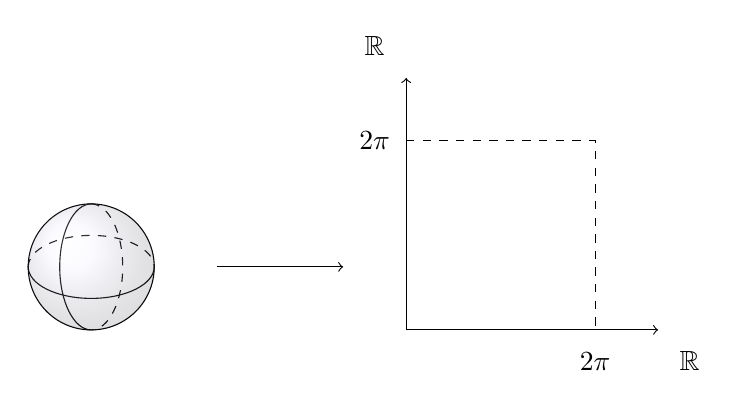
\begin{tikzpicture}[scale=0.8]
    \draw (-1,0) arc (180:360:1cm and 0.5cm);
    \draw[dashed] (-1,0) arc (180:0:1cm and 0.5cm);
    \draw (0,1) arc (90:270:0.5cm and 1cm);
    \draw[dashed] (0,1) arc (90:-90:0.5cm and 1cm);
    \draw (0,0) circle (1cm);
    \shade[ball color=blue!10!white,opacity=0.20] (0,0) circle (1cm);
    \draw[->] (2,0) -- (4,0);
\draw[->] (5,-1) node (v1) {} -- (5,3);
\draw[->] (5,-1) -- (9,-1);
\draw[dashed] (5,2) -- (8,2) -- (8,-1);
\node at (4.5,3.5) {$\mathbb{R}$};
\node at (9.5,-1.5) {$\mathbb{R}$};
\node at (4.5,2) {$2\pi$};
\node at (8,-1.5) {$2\pi$};
\end{tikzpicture}
\end{center}
\caption{Illustration of the 3-dimensional hypersphere, with a search space of $\mathbb{R}^2$
\label{fig:searchInAngles}}
\end{figure}




\clearpage
\subsection{Tetris configuration}

Section about better featuresets and normal tetris instead of hard tetris
for finding the optimal settings.





\clearpage

\bibliography{BSc2014}
\bibliographystyle{apalike}

\clearpage

\begin{appendices}

\section{Experiments}
This appendix contains all of the included experiments from which we have derived our results. Each of the plots, depending on the number of experiments, will depict the mean scores of the experiments or the experiments themselves.\\
With each experiment, a table detailing the parameter values will be included for others who would want to reproduce these experiments. Depending on the optimizer (weather it is Cross Entropy or CMA), the table will contain some custom rows, unique for the specific algorithm.\\
Similar for all experiments is the 30 games played with the new mean of each generation to generate the learning curve.\\
The tables are formatted 
\begin{table}[h]
\centering
\caption{Overview of the two table formats}
\begin{tabular}{l r}
Optimizer & -\\
Number of Evaluations & -\\
Number of Learning Games & -\\
Population size& -\\
Parent size & -\\
Games per Agent & -\\
Tetris Type & -\\
\hline
Recombination Type & -\\
Initial Sigma & -
\end{tabular}
\quad
\begin{tabular}{l r}
Optimizer & -\\
Number of Evaluations & -\\
Number of Learning Games & -\\
Population size & -\\
Parent size & -\\
Games per Agent & -\\
Tetris Type & -\\
\hline
Sigma & -\\
Noise Type & -\\
Noise & -
\end{tabular}
\end{table}

\clearpage

\subsection{Verification of Cross Entropy}
Using the same configuration as in "reference paper", we will reproduce the experiments to verify our implementation of Cross Entropy into the Shark Library.\\
\\
\begin{table}[h!]
\centering
\caption{Cross Entropy - No noise}
\begin{tabular}{l r}
Optimizer & Cross Entropy\\
Number of Evaluations & 8000\\
Population size & 100\\
Parent size & 10\\
Games per Agent & 1\\
Tetris Type & Normal\\
\hline
Sigma & 100\\
Noise Type & No noise\\
Noise & -
\end{tabular}
\end{table}

\begin{table}[h!]
\centering
\caption{Cross Entropy - Constant noise}
\begin{tabular}{l r}
Optimizer & Cross Entropy\\
Number of Evaluations & 8000\\
Population size & 100\\
Parent size & 10\\
Games per Agent & 1\\
Tetris Type & Normal\\
\hline
Sigma & 100\\
Noise Type & Constant\\
Noise & 4
\end{tabular}
\end{table}

\begin{table}[h!]
\centering
\caption{Cross Entropy - Linear decreasing noise}
\begin{tabular}{l r}
Optimizer & Cross Entropy\\
Number of Evaluations & 8000\\
Population size & 100\\
Parent size & 10\\
Games per Agent & 1\\
Tetris Type & Normal\\
\hline
Sigma & 100\\
Noise Type & Linear decreasing\\
Noise & $max \left( 5 - \frac{t}{10}, 0 \right)$
\end{tabular}
\end{table}


\clearpage

\subsection{Population and selection size}
We want to investigate if there exists a better configuration than the 100/10 which was also previously used by other researchers.\\
In Cross Entropy for the Tetris problem, 10 \% Parent selection is used as standard. However, we will also test 50 \% Parent selection is a configuration from CMA which we will also test.\\
The general testing parameters are as follows
\begin{table}[h]
\centering
\caption{General setup for Population/Parent size}
\begin{tabular}{l r}
Optimizer & Cross Entropy\\
Number of Evaluations & 8000\\
Population size & See table \ref{CEPopulationParentSize}\\
Parent size & See table \ref{CEPopulationParentSize}\\
Games per Agent & 1\\
Tetris Type & Normal\\
\hline
Sigma & 100\\
Noise Type & Constant\\
Noise & 4
\end{tabular}
\end{table}

with the following population/Parent size

\begin{table}[h]
\centering
\caption{Population/Parent size \label{CEPopulationParentSize}}
\begin{tabular}{l l}
Population size & Parent size\\
\hline
10 & 1\\
10 & 5\\
22 & 2\\
22 & 11\\
50 & 5\\
50 & 25\\
100 & 10\\
100 & 50\\
200 & 20\\
200 & 100
\end{tabular}
\end{table}

INSERT PLOTS HERE.\\
\\
quantile table and two graphs over the mean plots of 10 \% and 50 \% Parent size

\clearpage



\subsection{Optimal settings for Cross Entropy - Games per agent}
Experiment to determine the optimal number of games played per agent for best resulting score at lowest evaluation cost.

\begin{table}[h]
\centering
\caption{General setup for Population/Parent size}
\begin{tabular}{l r}
Optimizer & Cross Entropy\\
Number of Evaluations & 80000\\
Population size & See table \ref{GamesPerAgentCE}\\
Parent size & See table \ref{GamesPerAgentCE}\\
Games per Agent & See table \ref{GamesPerAgentCE}\\
Tetris Type & Normal\\
\hline
Sigma & 100\\
Noise Type & Constant\\
Noise & 4
\end{tabular}
\end{table}

with the following population/Parent size and number of games played per agent

\begin{table}[H]
\centering
\begin{tabular}{c c c}
Population Size & Parent size & Games per Agent\\
\hline
$10$ & $10\%$ & 1/3/5/7/10\\
$10$ & $50\%$ & 1/3/5/7/10\\
$22$ & $10\%$ & 1/3/5/7/10\\
$22$ & $50\%$ & 1/3/5/7/10\\
$50$ & $10\%$ & 1/3/5/7/10\\
$50$ & $50\%$ & 1/3/5/7/10\\
$100$ & $10\%$  & 1/3/5/7/10\\
$100$ & $50\%$ & 1/3/5/7/10\\
$200$ & $10\%$ & 1/3/5/7/10\\
$200$ & $50\%$ & 1/3/5/7/10
\end{tabular}
\caption{Games per agent CE experiment setup\label{GamesPerAgentCE}}
\end{table}

INSERT PLOTS HERE.\\
\\
quantile table and two graphs over the mean plots

\clearpage

\subsection{Optimal settings for CMA - Initial Step-size}
Experiments to find the best initial step-size for CMA.

\begin{table}[h]
\centering
\caption{Overview of the two table formats}
\begin{tabular}{l r}
Optimizer & CMA\\
Number of Evaluations & 8000\\
Number of Learning Games &30\\
Population size& 13\\
Parent size & 6\\
Games per Agent & 1\\
Tetris Type & Normal\\
\hline
Recombination Type & Superlinear\\
Initial Sigma & See table \ref{InitialSigmaTest}
\end{tabular}
\end{table}

with the following initial sigma

\begin{table}[H]
\centering
\begin{tabular}{c | c c c c c c}
$\sigma_0$ & 0.1 & 0.2 & 0.5 & 0.8 & 1.0
\end{tabular}
\caption{Initial sigma configurations \label{InitialSigmaTest}}
\end{table}

INSERT PLOTS HERE.\\
\\


\begin{figure}[H]
\centering
\begin{tabular}{r | r r r r r}
$\sigma_0$ & mean & Q1 & Q2 & Q3\\
\hline
0.1 & 50769.3 & 21301.1 & 54588.7 & 73972.4\\
0.2 & 42290.6 & 32180.2 & 42290.6 & 49337.4\\
0.5 & 53893.7 & 14211.1 & 66773.0 & 85816.7\\
0.8 & 37557.7 & 1422.8  & 15450.8 & 93719.4\\
1.0 & 49537.9 & 31369.8 & 49537.4 & 58454.6
\end{tabular}
\caption{Results of CMA-ES with adjusted initial step-size \label{CMAInitialSigmaConfigTest}}
\end{figure}

\clearpage

\subsection{Optimal settings for CMA - Experiment for finding the optimal settings}
Experiments finding the best configuration of population and parent size with recombination type. The parent size is dependent on the recombination type, therefore we tested these parameter together.
\begin{table}[h]
\centering
\caption{Overview of the two table formats}
\begin{tabular}{l r}
Optimizer & CMA\\
Number of Evaluations & 80000\\
Number of Learning Games &30\\
Population size& See table \ref{SuperCMAExperiment}\\
Parent size & See table \ref{SuperCMAExperiment}\\
Games per Agent & See table \ref{SuperCMAExperiment}\\
Tetris Type & Hard\\
\hline
Recombination Type & See table \ref{SuperCMAExperiment}\\
Initial Sigma & 1
\end{tabular}
\end{table}

\begin{table}[H]
\centering
\begin{tabular}{c c l c}
Population Size & Parent size & Recombination Type & Games per Agent\\
\hline
$12$ & $1$ & EQUAL/LINEAR/SUPERLINEAR & 1/3/5/7/10\\
$12$ & $3$ & EQUAL & 1/3/5/7/10\\
$12$ & $6$ & LINEAR/SUPERLINEAR & 1/3/5/7/10\\
$22$ & $2$ & EQUAL/LINEAR/SUPERLINEAR & 1/3/5/7/10\\
$22$ & $5$ & EQUAL & 1/3/5/7/10\\
$22$ & $11$ & LINEAR/SUPERLINEAR & 1/3/5/7/10\\
$50$ & $5$ & EQUAL/LINEAR/SUPERLINEAR & 1/3/5/7/10\\
$50$ & $12$ & EQUAL & 1/3/5/7/10\\
$50$ & $25$ & LINEAR/SUPERLINEAR & 1/3/5/7/10\\
$100$ & $10$ & EQUAL/LINEAR/SUPERLINEAR & 1/3/5/7/10\\
$100$ & $25$ & EQUAL & 1/3/5/7/10\\
$100$ & $50$ & LINEAR/SUPERLINEAR & 1/3/5/7/10
\end{tabular}
\caption{Full experiments overview \label{SuperCMAExperiment}}
\end{table}


\clearpage

\subsection{Comparison - Initial comparison}
Comparison between the verified Cross Entropy and Shark (reference to shark) stock setting CMA.

\begin{table}[h]
\centering
\small
\caption{Shark stock CMA and Verified Cross Entropy}
\begin{tabular}{l r}
Optimizer & CMA\\
Number of Evaluations & 8000\\
Number of Learning Games & 30\\
Population size& 13\\
Parent size & 6\\
Games per Agent & 1\\
Tetris Type & Normal\\
\hline
Recombination Type & Superlinear\\
Initial Sigma & (what is stock)\\
\quad & \quad
\end{tabular}
\quad
\begin{tabular}{l r}
Optimizer & Cross Entropy\\
Number of Evaluations & 8000\\
Number of Learning Games & 30\\
Population size & 100\\
Parent size & 10\\
Games per Agent & 1\\
Tetris Type & Normal\\
\hline
Sigma & 100\\
Noise Type & Constant\\
Noise & 4
\end{tabular}
\end{table}

INSERT PLOTS HERE.

\clearpage

\subsection{Comparison - Comparison of featuresets}
Experiments to test Bertsekas and Dellacherie featuresets in regards to achieved score. This will tell if a different featureset affects the algorithms performance. If the behaviour is the same, then the Tetris complexity problem

\begin{table}[h]
\centering
\small
\caption{Shark stock CMA and Verified Cross Entropy}
\begin{tabular}{l r}
Optimizer & CMA\\
Number of Evaluations & 8000\\
Number of Learning Games & 30\\
Population size& 13\\
Parent size & 6\\
Games per Agent & 1\\
Tetris Type & Hard\\
\hline
Recombination Type & Superlinear\\
Initial Sigma & (what is stock)\\
\quad & \quad
\end{tabular}
\quad
\begin{tabular}{l r}
Optimizer & Cross Entropy\\
Number of Evaluations & 8000\\
Number of Learning Games & 30\\
Population size & 100\\
Parent size & 10\\
Games per Agent & 1\\
Tetris Type & Hard\\
\hline
Sigma & 100\\
Noise Type & Constant\\
Noise & 4
\end{tabular}
\end{table}

Used on the bertsekas and Dellacherie featuresets

INSERT PLOTS HERE.

\section{CMA initial step-size \label{appendixCMAInitialSigma}}

Shows the graps of the configuration test, with initial sigma
settings.

 - \comment{Insert in above section}

\section{Cross Entropy configuration settings \label{appendixCrossEntropyConfig}}

The plots from the configuration of cross entropy.
All plots shows the numbers of games played along the x-axis
and the mean score of the centroid agent along the y-axis.

\begin{tabular}{@{}l@{}l@{}}
\plotCEConfig{10}{1}{ce_ConstantNoise_l10_o1_} &
\plotCEConfig{10}{5}{ce_ConstantNoise_l10_o5_}
\end{tabular}

\begin{tabular}{@{}l@{}l@{}}
\plotCEConfig{22}{2}{ce_ConstantNoise_l22_o2_} &
\plotCEConfig{22}{11}{ce_ConstantNoise_l22_o11_}
\end{tabular}

\begin{tabular}{@{}l@{}l@{}}
\plotCEConfig{50}{5}{ce_ConstantNoise_l50_o5_} &
\plotCEConfig{50}{25}{ce_ConstantNoise_l50_o25_}
\end{tabular}

\begin{tabular}{@{}l@{}l@{}}
\plotCEConfig{200}{20}{ce_ConstantNoise_l10_o1_} &
\plotCEConfig{200}{100}{ce_ConstantNoise_l10_o5_}
\end{tabular}





 - \comment{Insert in above section}

\clearpage

\section{Cross Entropy Implementation - Shark library}

\subsection{CrossEntropyMethod.h}

\lstinputlisting[language=c++, style=customc]{CrossEntropyMethod.h}

\clearpage

\subsection{CrossEntropyMethod.cpp}

\lstinputlisting[language=c++, style=customc]{CrossEntropyMethod.cpp}


\end{appendices}


\end{document}